\documentclass[10pt]{article}
\usepackage[T1]{fontenc}
\usepackage[utf8]{inputenc}
\usepackage[margin=0.85in]{geometry}
\usepackage{amsmath,amssymb}
\usepackage{booktabs}
\usepackage{array}
\usepackage{tabularx}
\usepackage{graphicx}
\usepackage{float}
\usepackage{xcolor}
\usepackage{tcolorbox}
\usepackage{hyperref}
\graphicspath{{figures/}}

\newcommand{\code}[1]{\texttt{#1}}
\newtcolorbox{basic}[1][]{colback=green!4,colframe=green!40!black,title={In plain words},fonttitle=\bfseries,#1}
\newtcolorbox{advanced}[1][]{colback=blue!3,colframe=blue!40!black,title={The precise version},fonttitle=\bfseries,#1}

\title{Machine-Learning Models for Optimizing Skipper-CCD Operating Parameters:\\
What They Do, What They Need, and Whether They Should See the Full Trace}
\author{ML-assisted optimization of CCD operating parameters --- working note (draft)}
\date{14 October 2026 (first round of models)}

\begin{document}
\maketitle

\begin{abstract}
This note describes the models that will learn from the data packets: what they take in, what they predict, how they are
trained and checked, and how much data each needs. Each model is explained twice, in plain words and precisely. It then
addresses two design questions. Should a model be given the full trace, the hand-made trace features, or both? And can a
model find useful properties of the trace that we did not think of?

All models are implemented in \code{src/ml/} and were compared on a \emph{synthetic} CCD world built to mimic the packets
(\code{src/ml/synthetic.py}). The synthetic results compare methods only; they say nothing about the real CCD. The real
comparison will be repeated on the first scan.
\end{abstract}

\tableofcontents

%======================================================================
\section{Summary}

\begin{basic}
\begin{itemize}
\item \textbf{What the models do.} A packet gives, for one choice of settings, cheap measurements (traces, a few minutes) and an
  expensive one: the image, whose WADERs fit gives the read noise $\sigma_e$, the dark charge $\lambda$ and the gain. The models
  learn how these three numbers depend on the settings and on what the traces show.
\item \textbf{Two jobs.} The \emph{predictor} looks at a packet's traces and says what the image would show (a ``virtual image'')
  with an error bar. The \emph{surrogate} looks only at the settings and is used to choose the next settings to try (Bayesian
  optimization).
\item \textbf{Which models.} The surrogate is a Gaussian process: it works with tens to a few hundred packets and knows how sure it
  is. For the predictor, Gaussian processes and gradient-boosted trees on the hand-made features come first. Neural networks
  that read the trace curves come once there are enough packets, or when they are pre-trained on the many unlabeled
  traces.
\item \textbf{Full trace or features?} Both, in layers. The hand-made features are the main input. The trace \emph{curves} (mean
  skip waveform, transfer shapes, noise spectra) go to a network that can learn its own features. The raw 3-million-sample trace
  is not given directly: it is mostly repetitions of the same cycle, and the curves keep its information in a compact form.
\item \textbf{Can a model find features we missed?} Yes, if it is given the curves (or the folded trace) and enough data. On the
  synthetic world, a network on the curves found an intermittent noise floor that is missing from the hand-made list: $\sigma_e$ error
  1.9\,\% at 480 packets, against $\sim$11\,\% for every model on the hand-made features.
\item \textbf{Data.} One scan of 10 parameters $\times$ 20 values (241 packets, about 76\,h) is enough for the surrogate and the
  feature-based predictor; they are useful from $\sim$60 packets. In the synthetic tests, the network on the curves overtook them between
  240 and 480 labeled packets. Pre-training on unlabeled traces (a scan produces $\sim$30{,}000) should lower that.
\item \textbf{Reference traces matter}: the dark charge drifts with the CCD state. Settings alone predict it to $\sim$25\,\%; with the reference
  traces it is 3.6\,\%.
\item \textbf{A new module} needs about 20 of its own packets before any first-round model predicts it well.
\item \textbf{Second round} (Section~\ref{sec:proto}). SUMMARY-PROTO-PLACEHOLDER
\item \textbf{Real data} (Sections~\ref{sec:realtest}--\ref{sec:format}): a staged test plan; the packets need no extra time, but per-row
  $\lambda$ from WADERs, a scan design with joint changes, trace-only packets, recorded conditions and 2--5 packets per new module would help;
  and a set of linked tables (per trace set, curves, labels with errors, image rows) instead of one flat \code{dataset.csv}.
\end{itemize}
\end{basic}

%======================================================================
\section{The problem}

\begin{basic}
We can set about 40 knobs on the CCD electronics: bias voltages, clock levels and clock timing. Every combination gives an image
with some read noise, some dark charge and some gain. We want the knobs that give the lowest noise and dark charge. Trying a
combination costs about 16 minutes (a packet with an image), so we can try a few hundred, not millions. A model learns from the
combinations tried so far how the result depends on the knobs, and suggests where to look next. The traces make each try more
informative: in a minute they show how the clocks, the amplifier and the noise behave right now.
\end{basic}

\begin{advanced}
Let $\theta \in \mathbb{R}^d$ be the operating parameters ($d \approx 10$ after grouping pins, up to $\sim$40), $a$ the amplifier
and $z$ the unobserved state of the CCD and electronics (temperature, history, drifts). The image gives noisy labels
\begin{equation}
y = \bigl(\log\sigma_e,\ \log\lambda,\ \log g\bigr) = f(\theta, a, z) + \varepsilon,\qquad \varepsilon \sim \mathcal N(0, \Sigma_\text{label}),
\end{equation}
with label noise of about 1.5\,\% ($\sigma_e$), 3\,\% ($\lambda$) and 0.8\,\% ($g$) for the 16-row image (\code{docs/packet\_design.md}).
Logs are used because all three quantities are positive and an error in the log is a relative error.
The traces give a feature vector $x = h(\theta, a, z) + \eta$ at $\theta$, and $x_\text{ref} = h(\theta_\text{ref}, a, z) + \eta'$ at
the reference, taken in the same packet. The goal is
\begin{equation}
\theta^\star = \arg\min_{\theta \in \Theta_\text{allowed}} \; J(\theta),\qquad J = \log\sigma_e + w\,\log\lambda ,
\end{equation}
or a multi-objective version (the Pareto front of $\sigma_e$ and $\lambda$). $\Theta_\text{allowed}$ is set by the voltage
limits and the relations between parameters.
\end{advanced}

%======================================================================
\section{The two jobs: predictor and surrogate}

\begin{figure}[H]
\centering
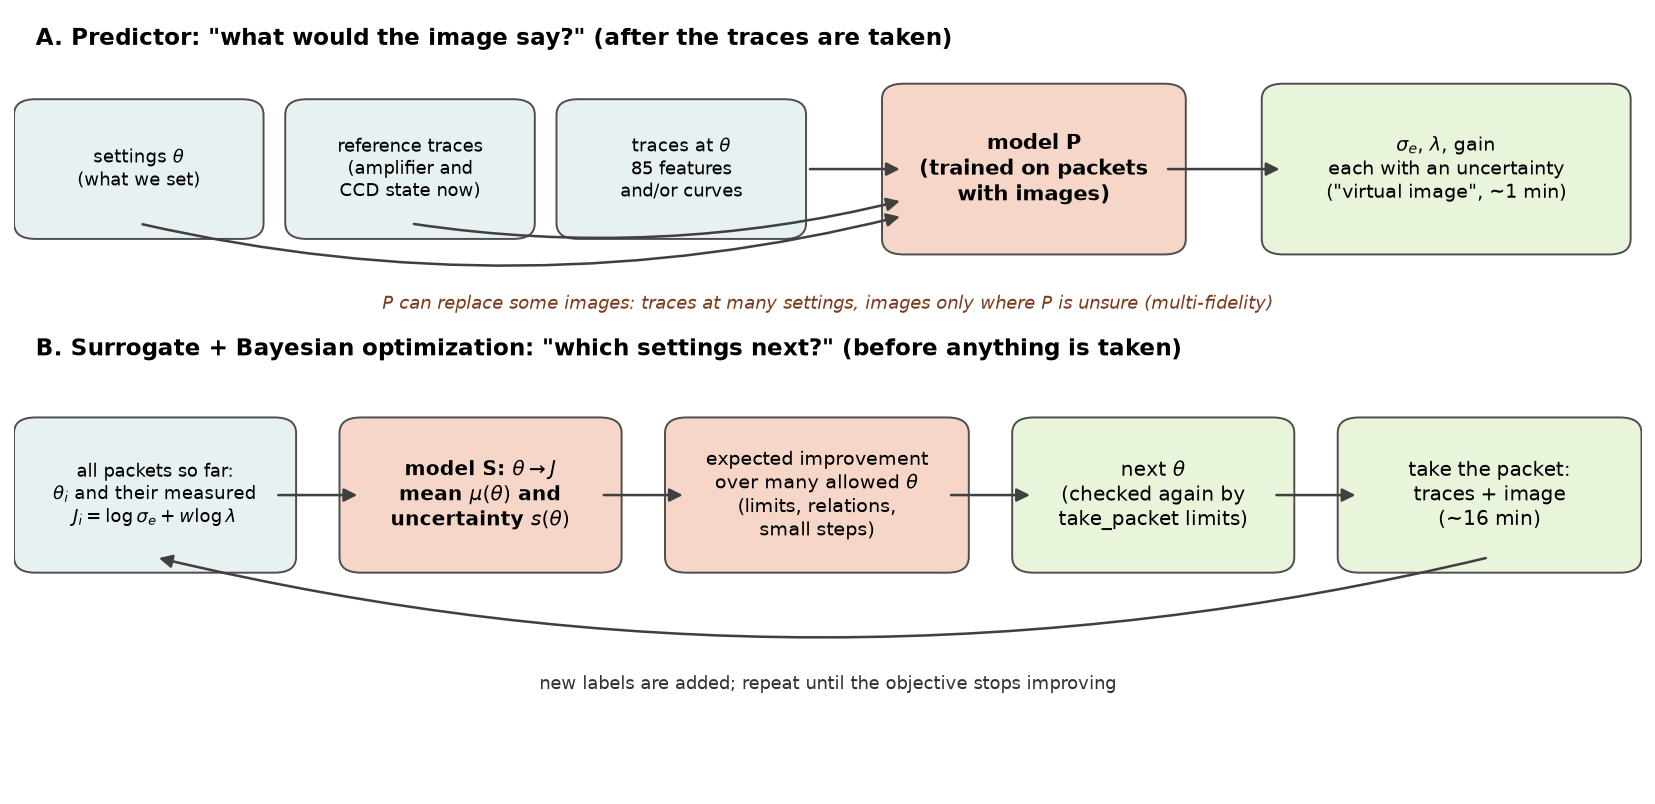
\includegraphics[width=\textwidth]{ml_roles.png}
\caption{The two roles. A: the predictor $P$ turns a packet's traces (and settings) into predicted image labels. B: the
surrogate $S$ maps settings to the objective, and Bayesian optimization uses its mean and uncertainty to choose the next
settings.}
\label{fig:roles}
\end{figure}

\begin{basic}
\textbf{Predictor $P$.} \emph{After} a packet's traces are taken, $P$ says what the image would show. This is useful because
traces take a minute and images a quarter of an hour. Settings could be screened with traces only, and images taken
only where $P$ is unsure. It also uses the reference traces, which tell it which amplifier it is looking at and how the CCD
is doing today.

\textbf{Surrogate $S$.} \emph{Before} anything is measured, $S$ guesses the result at settings never tried, and how unsure it is.
The optimizer picks the next settings where the guess is good or the uncertainty is large. $S$ cannot use traces at new
settings, because they do not exist yet.
\end{basic}

\begin{advanced}
\begin{itemize}
\item $P(\theta, a, x, x_\text{ref}) \rightarrow (\hat y, \hat\sigma_y)$ is a regression with heteroscedastic uncertainty.
  $x_\text{ref}$ identifies the amplifier (it generalizes to amplifiers never seen, unlike an amplifier one-hot) and estimates the
  state $z$, which $\theta$ cannot. $\Delta x = x - x_\text{ref}$ removes the amplifier's own signature.
\item $S(\theta, a) \rightarrow (\mu_J(\theta), s_J(\theta))$ is a probabilistic surrogate, normally a Gaussian process. The
  acquisition (Section~\ref{sec:bo}) needs a calibrated $s_J$.
\item \textbf{Multi-fidelity:} traces are a cheap, correlated fidelity of the labels. A co-kriging or multi-task GP can use
  trace-only packets ($x$ at many $\theta$) together with full packets ($x$ and $y$ at fewer $\theta$). This is the natural extension
  once $P$ is shown to work.
\end{itemize}
\end{advanced}

%======================================================================
\section{What goes in and what comes out}

\begin{table}[H]
\centering
\small
\begin{tabularx}{\textwidth}{>{\raggedright\arraybackslash}p{2.6cm}>{\raggedright\arraybackslash}p{4.6cm}Xc}
\toprule
Input group & Content & Why & Size \\
\midrule
\code{theta}, \code{delta} & the operating parameters; their change from the reference & what we control & 10--40 \\
\code{amp} & which amplifier (one-hot of board and channel) & amplifiers differ by 4$\times$ in noise and 2$\times$ in gain & 4--8 \\
\code{trace} & the 85 hand-made features at $\theta$, mean over the trace sets & how the clocks, amplifier and noise behave & 85 \\
\code{ref} & the same at the reference, minutes earlier in the same packet & the amplifier's identity and the CCD state now & 85 \\
\code{diff} & \code{trace} $-$ \code{ref} & the change the settings caused & 85 \\
\code{trace\_sd} & the scatter of each feature over the trace sets & how much to trust each feature & 85 \\
curves & 12 curves: mean skip waveform, H/V transfer shapes, CDS pattern, autocorrelation, Allan deviation, spectra, noise vs window length, equivalent-time pulse, variation along the cycle & room for features nobody has defined & 4{,}187 \\
CDS matrix & the CDS of every pixel and skip & skip-to-skip structure & 5{,}000 \\
raw trace & every ADC sample & everything & $3\times10^6$ \\
\midrule
\textbf{Outputs} & $\log\sigma_e$, $\log\lambda$, $\log g$ per amplifier, each with a standard deviation; or $J$ for the surrogate & & 3 \\
\bottomrule
\end{tabularx}
\caption{Model inputs. All are in \code{dataset.csv} or the \code{.npz} files written by \code{process\_packet.py}; \code{src/ml/data.py}
builds any combination (\code{make\_inputs}, \code{curve\_tensor}, \code{curves\_from\_processed}).}
\label{tab:inputs}
\end{table}

\paragraph{One training example} is one amplifier in one packet: its settings, its features or curves, and its three labels.
A packet with 4 working amplifiers gives 4 examples. The examples of one packet share the CCD state and must stay together
when the data are split for testing.

%======================================================================
\section{The model families}

Table~\ref{tab:families} lists the five families in \code{src/ml/models.py}. All have the same interface
(\code{fit(X, Y)}, \code{predict(X)} $\rightarrow$ mean, std) and standardize their inputs using the training rows only.

\begin{table}[H]
\centering
\small
\begin{tabularx}{\textwidth}{>{\raggedright\arraybackslash}p{2.6cm}X>{\raggedright\arraybackslash}p{3.0cm}>{\raggedright\arraybackslash}p{2.7cm}}
\toprule
Model & Idea & Strengths & Labeled packets \\
\midrule
Bayesian ridge & a weighted sum of the inputs & baseline; readable; never wild & 20+ \\
Gradient-boosted trees & a sum of hundreds of small yes/no decision trees & nonlinear; robust to scale and outliers; feature importances & 100+ \\
Gaussian process & a smooth function; predictions are similarity-weighted averages of the examples & calibrated uncertainty; best with little data; drives Bayesian optimization & 20--1000 \\
Neural-net ensemble & 5 small networks, each predicts a value and its variance & smooth nonlinear; scales to many examples & 300+ \\
1D CNN on curves & filters slide along the curves and learn which shapes matter & finds its own features & 500+ (fewer with pre-training) \\
\bottomrule
\end{tabularx}
\caption{The model families.}
\label{tab:families}
\end{table}

\subsection{Bayesian ridge (linear)}
\begin{basic}
Each output is a weighted sum of the inputs; the weights are learned. ``Bayesian'' means the weights are kept small unless the data
insist, and the model reports how sure it is. It cannot represent an optimum (a noise minimum in VDD), so it serves as the
yardstick the other models must beat.
\end{basic}
\begin{advanced}
$y = w^\top \tilde x + b + \varepsilon$, with standardized inputs $\tilde x$, prior $w \sim \mathcal N(0, \alpha^{-1} I)$ and noise
$\varepsilon \sim \mathcal N(0, \beta^{-1})$. $\alpha$ and $\beta$ maximize the marginal likelihood. The predictive variance is
$\beta^{-1} + \tilde x^\top \Sigma_w \tilde x$.
\end{advanced}

\subsection{Gradient-boosted trees}
\begin{basic}
A decision tree asks a few yes/no questions (``is VDD below $-19.4$?'', ``is the H-transfer minimum deeper than $-10^5$?'') and
returns a number. Boosting adds a few hundred small trees, each correcting the errors of the ones before. Trees handle thresholds,
different scales and irrelevant inputs well. The error bar comes from two extra models that predict the 16\,\% and 84\,\% quantiles.
\end{basic}
\begin{advanced}
$\hat y(x) = \sum_{m=1}^{M} \nu\, t_m(x)$, with depth-limited regression trees $t_m$ fitted to the gradient of the loss at stage $m$
(histogram-based, \code{HistGradientBoostingRegressor}; $M = 300$, $\nu = 0.05$, 15 leaves, $\geq 10$ examples per leaf). The
uncertainty is $\hat\sigma = (\hat q_{0.84} - \hat q_{0.16})/2$ from quantile (pinball) losses. These quantile estimates are noisy with few
examples (Section~\ref{sec:results}).
\end{advanced}

\subsection{Gaussian process}
\begin{basic}
A Gaussian process predicts at new settings by averaging the examples it has seen, weighting each by how similar its settings are.
Far from all examples the prediction falls back to the average and the error bar grows. That is exactly the honesty an optimizer needs
(``I have not looked there''). It learns one ``similarity distance'' per input: inputs that do not matter get a huge distance and are
ignored. These distances show which settings and features matter.
\end{basic}
\begin{advanced}
$f \sim \mathcal{GP}(m, k)$ with
\begin{equation}
k(x, x') = c\;\mathrm{Mat\acute ern}_{5/2}\!\left(r\right) + \sigma_n^2\,\delta_{xx'},\qquad
r^2 = \sum_i \frac{(x_i - x'_i)^2}{\ell_i^2},
\end{equation}
one length scale $\ell_i$ per input (automatic relevance determination). With $K$ the kernel matrix of the training inputs,
\begin{equation}
\mu(x_*) = k_*^\top (K + \sigma_n^2 I)^{-1} y,\qquad
s^2(x_*) = k(x_*, x_*) - k_*^\top (K + \sigma_n^2 I)^{-1} k_* .
\end{equation}
$c$, $\ell_i$ and $\sigma_n$ maximize the log marginal likelihood
$-\tfrac12 y^\top (K+\sigma_n^2 I)^{-1} y - \tfrac12 \log|K+\sigma_n^2 I| - \tfrac n2 \log 2\pi$. The cost is $O(n^3)$, so above
$\sim$400--800 examples a subset or a sparse approximation is used. Relevance $= 1/\ell_i$ (Figure~\ref{fig:relevance}).
\end{advanced}

\subsection{Neural-network ensemble}
\begin{basic}
A small neural network is a flexible curve-fitter with a few thousand adjustable numbers. Five of them are trained from different
random starts. Where they agree, the prediction is trusted; where they disagree, the error bar grows. Each network also predicts its
own error bar, which captures noise that no input explains.
\end{basic}
\begin{advanced}
Each member $j$ has two hidden layers of 64 units (SiLU) and outputs $(\mu_j, \log\sigma_j^2)$. It is trained with the Gaussian
negative log-likelihood $\tfrac12\log\sigma_j^2 + (y-\mu_j)^2/2\sigma_j^2$, with AdamW, weight decay $10^{-3}$ and early stopping on 15\,\%
of the training packets. The ensemble ``deep ensemble'' predicts $\mu = \bar\mu_j$ and
$s^2 = \overline{\sigma_j^2} + \mathrm{Var}_j(\mu_j)$ (aleatoric plus epistemic uncertainty).
\end{advanced}

\subsection{1D convolutional network on the trace curves}
\begin{basic}
This model gets the curves themselves, not numbers computed from them. It slides small learned ``templates'' (filters) along each
curve. It does not decide in advance where the reset pulse is or what a noise floor looks like: it finds the shapes that help predict
the labels. Settings and hand-made features can be added at the end, so it has both.
\end{basic}
\begin{advanced}
The curves are resampled to $L = 256$ points (spectra and Allan deviations in log) and stacked as channels, $C \times L$. Each position
is standardized with the training rows. Three convolution blocks (kernel sizes 7, 7, 5; 16, 32, 32 filters; SiLU; max-pooling) are
followed by adaptive average pooling to $8 \times 32$. The scalar inputs are appended, and a dense layer (64) outputs $(\mu, \log\sigma^2)$
per target. It is trained like the ensemble above (3 members). About 14{,}000 weights; translation-equivariant filters suit curves
whose features move with the timing.
\end{advanced}

%======================================================================
\section{Full trace, hand-made features, or both?}
\label{sec:fulltrace}

\begin{figure}[H]
\centering
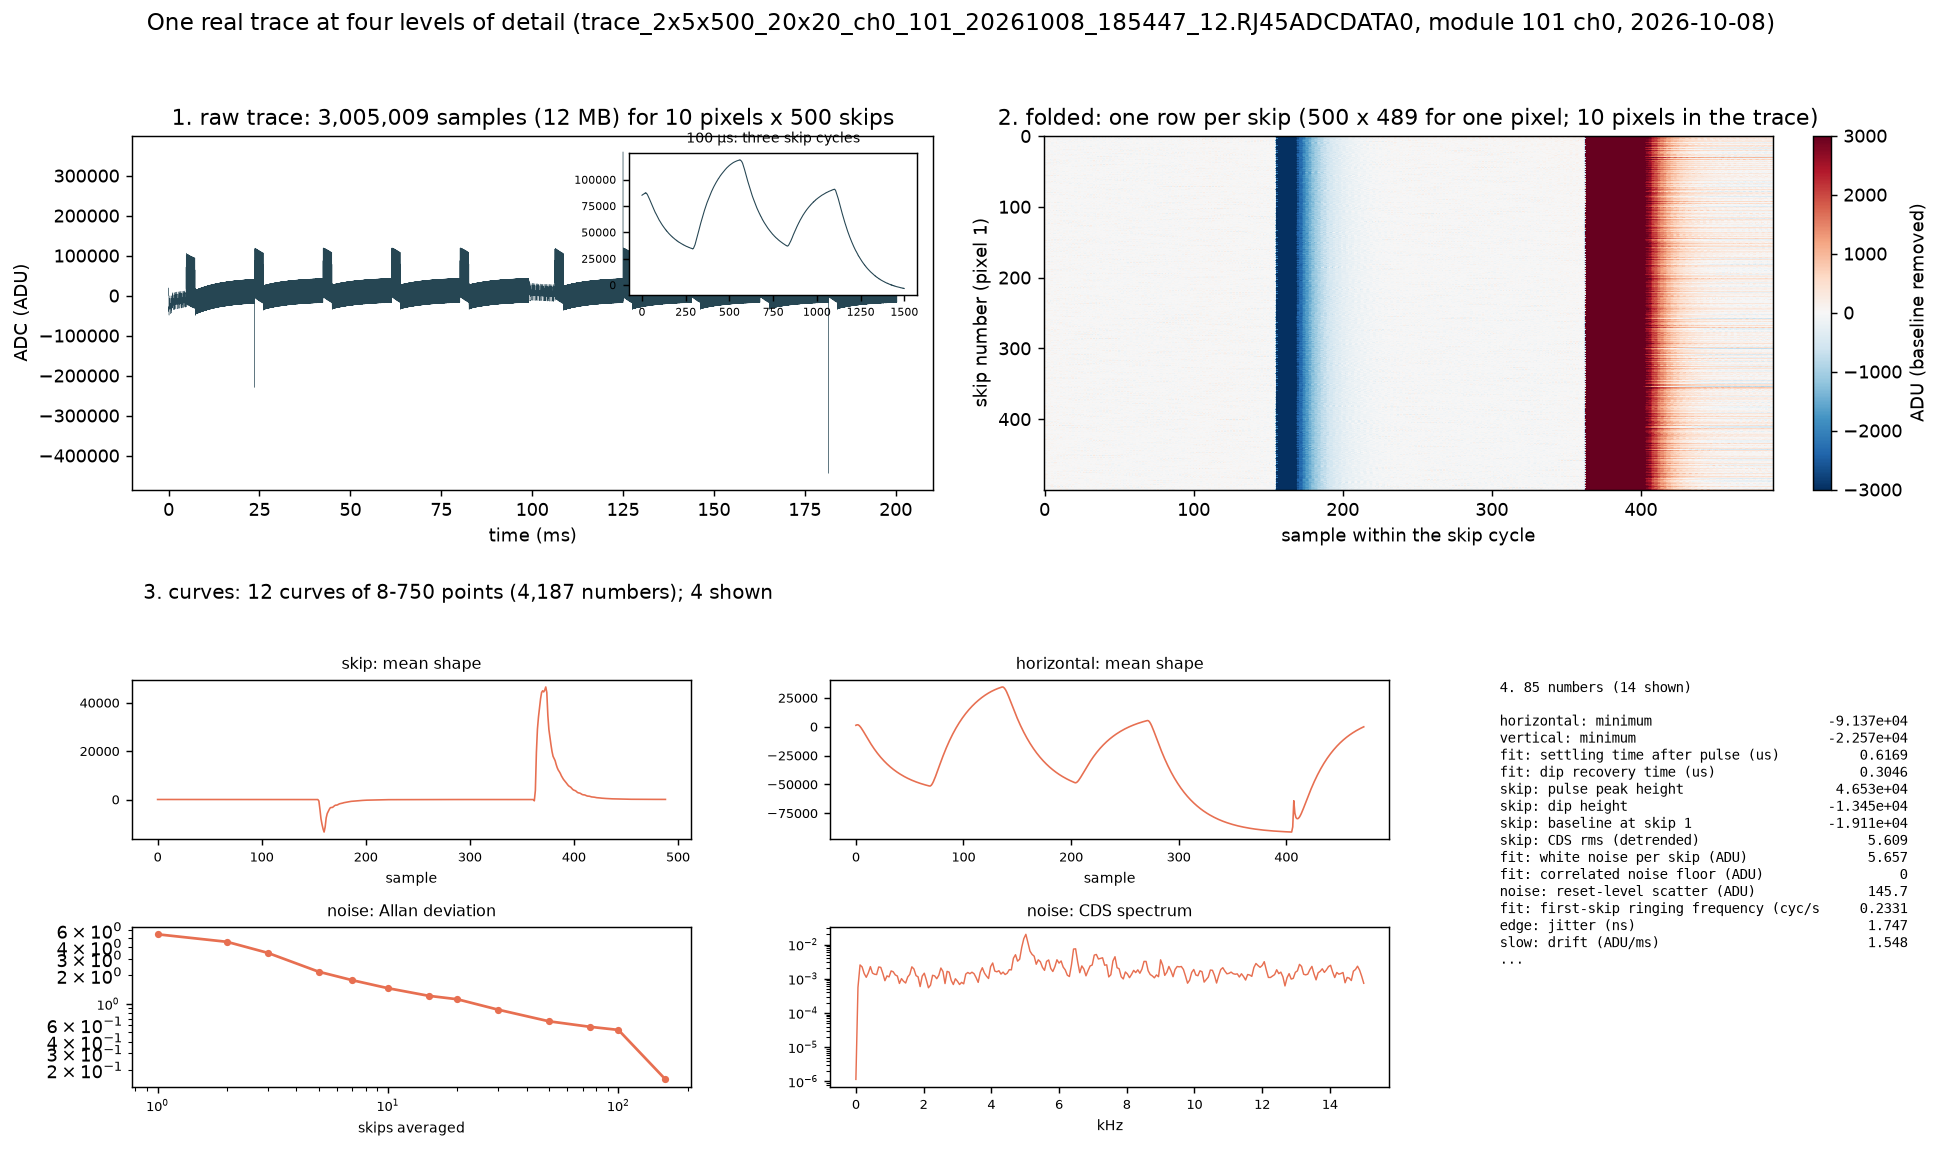
\includegraphics[width=\textwidth]{ml_representations.png}
\caption{One real trace (2026-10-08, module 101, channel 0) at four levels of detail: 3 million raw samples, the same samples folded
into skip cycles, the 12 curves, and the 85 numbers.}
\label{fig:representations}
\end{figure}

\subsection{What each level contains}
\begin{basic}
\begin{itemize}
\item The \textbf{raw trace} is mostly the same 33-microsecond skip cycle repeated 5{,}000 times, plus the transfers between pixels.
  Nearly all its 3 million numbers are repetitions.
\item \textbf{Folding} stacks the cycles on top of each other (Figure~\ref{fig:representations}, panel 2). Nothing is lost; it is just
  rearranged so that ``the same moment of the cycle'' lines up.
\item The \textbf{curves} average over the cycles (the mean waveform) or summarize how the cycles differ (spectra, Allan deviation,
  variation along the cycle). They keep almost everything that is systematic, in 4{,}000 numbers.
\item The \textbf{85 features} pick the parts of the curves we know to be meaningful: a pulse height, a time constant, a noise level.
\end{itemize}
\end{basic}

\begin{advanced}
Let the trace be $v_t$, $t = 1\dots T$ ($T \approx 3\times10^6$). With the exact cycle length $P$ (488.7 samples), the folded
array $V_{pk\tau} = v_{t_0(p) + kP + \tau}$ (pixel $p$, skip $k$, phase $\tau$) is a lossless re-indexing apart from the transfer
segments. The curves are mostly first and second moments of $V$ over $k$ and $p$: the mean $\bar V_\tau$; the variance along the
cycle $\mathrm{Var}_k V_{\cdot k\tau}$; and the spectrum and Allan deviation of the CDS series
$c_{pk} = \bar V_{pk,\text{ped}} - \bar V_{pk,\text{sig}}$. These are sufficient statistics if the trace is a stationary Gaussian
process within each phase; they drop only higher-order structure and rare events, and the 85 features summarize that remainder (outliers,
kurtosis, steps). The 85 features are fixed, nonlinear functionals of these curves.
\end{advanced}

\subsection{The trade-off}
\begin{basic}
More detail can only help \emph{if there are enough examples to learn from it}. A model has to learn what each input means. With
85 numbers and a few hundred packets that is feasible; with 3 million numbers per example it would memorize the training packets
instead of learning. The hand-made features are knowledge we put in so that the model does not need thousands of examples to discover
that the reset-pulse height matters.
\end{basic}

\begin{advanced}
For $n$ labeled examples and an input of dimension $p$, a flexible model's estimation error grows with its effective number of
parameters relative to $n$ (bias--variance; for linear models the excess risk is $\propto \sigma^2 p / n$). Here
$n \approx 10^3$ (241 packets $\times$ 4 amplifiers) and the 4 amplifiers of a packet are correlated (one CCD state). Rough data needs:
\begin{itemize}
\item 85 features: manageable, especially with priors (GP length scales, tree regularization);
\item the curves ($p \approx 4{,}000$ but highly structured): a CNN with weight sharing has $\sim 10^4$ weights; feasible at
  $n \sim 10^3$--$10^4$, or with pre-training;
\item the raw trace: needs $n \gg 10^4$ or a pre-trained encoder.
\end{itemize}
\end{advanced}

\subsection{Recommendation}
\begin{enumerate}
\item \textbf{Hand-made features (and $\theta$, $x_\text{ref}$, $\Delta x$) are the primary input} for the first models: they need
  the least data and are interpretable.
\item \textbf{Add the curves in a second model (CNN) and compare} on held-out packets. If the CNN wins, look at what it uses
  (Section~\ref{sec:own}) and turn it into a new hand-made feature where possible.
\item \textbf{Do not feed the raw trace directly.} Use the folded trace or the CDS matrix only through a pre-trained encoder (below),
  and only if the curves leave something unexplained.
\item \textbf{Keep everything.} \code{process\_packet.py} already saves the raw samples, the CDS matrix and the curves of every trace
  (\code{.npz}), so any representation can be tried later without new data.
\end{enumerate}

%======================================================================
\section{Can the model find its own features?}
\label{sec:own}

\begin{basic}
Yes, with three conditions:
\begin{enumerate}
\item \textbf{The information must be in what it sees.} A network on the 85 numbers can only combine those 85 numbers. A network on the
  curves can find any shape in the curves: a bump, a slope, a floor, a resonance.
\item \textbf{It needs enough examples} to tell a real pattern from chance.
\item \textbf{It needs a reason}: the pattern must help predict the labels. Patterns that do not matter for $\sigma_e$, $\lambda$ or the
  gain are ignored, even if they are real.
\end{enumerate}
The synthetic test (Section~\ref{sec:results}) hides one effect from the hand-made list on purpose: a noise floor that does not average
down with more skips. It is visible only in the Allan-deviation and spectrum curves. Models on the hand-made features cannot see it;
the network on the curves can, once it has enough examples.
\end{basic}

\begin{advanced}
\paragraph{Why convolutions can discover features.} A convolutional filter $w$ applied to a curve $u$ gives
$(w * u)_\tau = \sum_j w_j u_{\tau+j}$; after a nonlinearity and pooling, this is a learned, localized detector (``a steep drop here'',
``a flattening at large $n$''). Training adjusts the $w$ by gradient descent on the label loss, so detectors that predict the labels are
reinforced. Hand-made features are fixed detectors chosen by us; the network can learn the same ones (e.g.\ a pulse height) or others.

\paragraph{Seeing what it learned.}
\begin{itemize}
\item \emph{Saliency / occlusion}: the change of the prediction when a stretch of a curve is perturbed or masked shows which positions
  it uses.
\item \emph{Probing}: regress the network's internal features on the 85 hand-made features. What is not explained by them is new.
\item \emph{Ablation}: compare the CNN with and without the hand-made features as extra inputs (Section~\ref{sec:results}).
\end{itemize}

\paragraph{Using unlabeled traces (self-supervised pre-training).} Labels are scarce (one image per packet), but traces are not: a 241-packet scan
with 5 + 10 trace sets gives $241 \times 15 \times 8 \approx 29{,}000$ traces, plus the 2026-10-08/12 data. An encoder can be
trained without labels:
\begin{itemize}
\item to reconstruct masked parts of the curves (masked autoencoder);
\item to map two repeats of the same packet close together and different settings apart (contrastive learning);
\item or to predict $\theta$ from the trace, which is known for every trace.
\end{itemize}
The supervised models then start from these learned features and need far fewer labeled packets. This is the realistic route to
using the folded trace or the CDS matrix.

\paragraph{Limits.} With few labels a flexible model can latch onto artifacts that happen to correlate with the labels in one scan
(e.g.\ the drift of one night). Grouped validation on an independent scan (and on other days) is essential before trusting a
``new feature''.
\end{advanced}

%======================================================================
\section{Training data needed}
\label{sec:data}

\begin{table}[H]
\centering
\small
\begin{tabularx}{\textwidth}{>{\raggedright\arraybackslash}p{4.4cm}X}
\toprule
Requirement & Why \\
\midrule
\textbf{Labeled packets}: traces and an image at the same settings, close in time & every example needs inputs and labels from the same
CCD state \\
\textbf{A space-filling design} (random or Latin-hypercube in all scanned parameters), after a one-at-a-time screening & one-at-a-time
scans cannot separate interactions; random designs let every model see combinations \\
\textbf{Several values per parameter} over a range that moves $\sigma_e$ and $\lambda$ clearly & a parameter that changes nothing teaches
nothing \\
\textbf{The reference repeated} (every 5--10 packets) & label noise floor, drift, and the state $z$ \\
\textbf{All four amplifiers}, ideally more than one module & to learn what is common and to test on an amplifier never seen \\
\textbf{An independent test scan} (another night) & the only honest test of a model and of any ``discovered'' feature \\
\textbf{Labels with uncertainties and flags} (WADERs) & the models are trained on log-labels; flagged fits are left out \\
\bottomrule
\end{tabularx}
\end{table}

\paragraph{How many packets.} From the learning curves (Figure~\ref{fig:learning}; synthetic, so only indicative):
\begin{itemize}
\item the Gaussian process (surrogate and feature-based predictor) is useful from $\sim$30--60 packets;
\item the feature-based models level off at a few hundred packets;
\item the CNN on the curves matched them up to $\sim$240 packets and overtook them by 480 (when the curves hold information the features
  lack); pre-training should bring that down.
\end{itemize}
The 241-packet scan (10 parameters $\times$ 20 values, $\sim$76\,h) is enough for the first two. Bayesian optimization
(Section~\ref{sec:bo}) needs far fewer packets than a grid to find good settings.

%======================================================================
\section{Validation and uncertainty}

\begin{itemize}
\item \textbf{Grouped splits}: all amplifiers of a packet are in training or in test, never both (\code{evaluate.grouped\_cv}).
\item \textbf{Independent test scan}: train on one scan, test on another (here: another synthetic scan).
\item \textbf{Held-out amplifier}: train on three amplifiers, test on the fourth. This works only with reference-based inputs
  (Section~\ref{sec:results}).
\item \textbf{Scores}: relative error $\sqrt{\overline{(\hat y - y)^2}}$ in log; $R^2$; \emph{coverage}, the fraction of test points
  within $\hat y \pm \hat\sigma$, which should be 0.68; negative log-likelihood. Coverage tells whether the error bars can be trusted,
  which matters for the optimizer.
\end{itemize}

%======================================================================
\section{Optimization}
\label{sec:bo}

\begin{basic}
After each packet the surrogate is refitted. Thousands of candidate settings within the allowed region are scored by how much they are
expected to improve on the best result so far. That score is large where the prediction is good \emph{or} where the model is unsure, so
the search both exploits and explores. The best candidate is checked against the limits again and measured, and the loop repeats.
\end{basic}
\begin{advanced}
With incumbent $J^+ = \min_i J_i$ and $z = (J^+ - \mu(\theta))/s(\theta)$, the expected improvement is
\begin{equation}
\mathrm{EI}(\theta) = \bigl(J^+ - \mu(\theta)\bigr)\,\Phi(z) + s(\theta)\,\phi(z).
\end{equation}
It is maximized over random candidates drawn in the allowed box, filtered by the relational constraints (\code{allowed} hook; still to be
filled with the limits being compiled), optionally within a trust region $|\theta - \theta^+| \le \Delta$ (bounded voltage steps).
Extensions:
\begin{itemize}
\item batch proposals (several packets per refit);
\item multi-objective acquisition (expected hypervolume improvement for the $\sigma_e$--$\lambda$ front);
\item multi-fidelity acquisition that decides between a trace-only packet and a full packet.
\end{itemize}
\end{advanced}

%======================================================================
\section{Results on the synthetic world}
\label{sec:results}

\paragraph{The synthetic world} (\code{src/ml/synthetic.py}) has:
\begin{itemize}
\item 10 parameters with the real names and nominal values;
\item 4 amplifiers per board, one 4$\times$ noisier;
\item toy physics with optima, a forbidden region (\code{VDRAIN} within 2.5\,V of \code{VDD}) and trade-offs: lower H rails mean less
  charge-transfer loss but more clock-induced charge;
\item a slowly drifting hidden state (``temperature'') that changes $\lambda$ by $\pm$35\,\% and shifts a few trace features;
\item a hidden noise floor, visible only in the curves;
\item label noise and repeat scatter as measured.
\end{itemize}
Models are trained on one synthetic scan and tested on an independent one.

\subsection{Which inputs help (240 training packets)}

\begin{figure}[H]
\centering
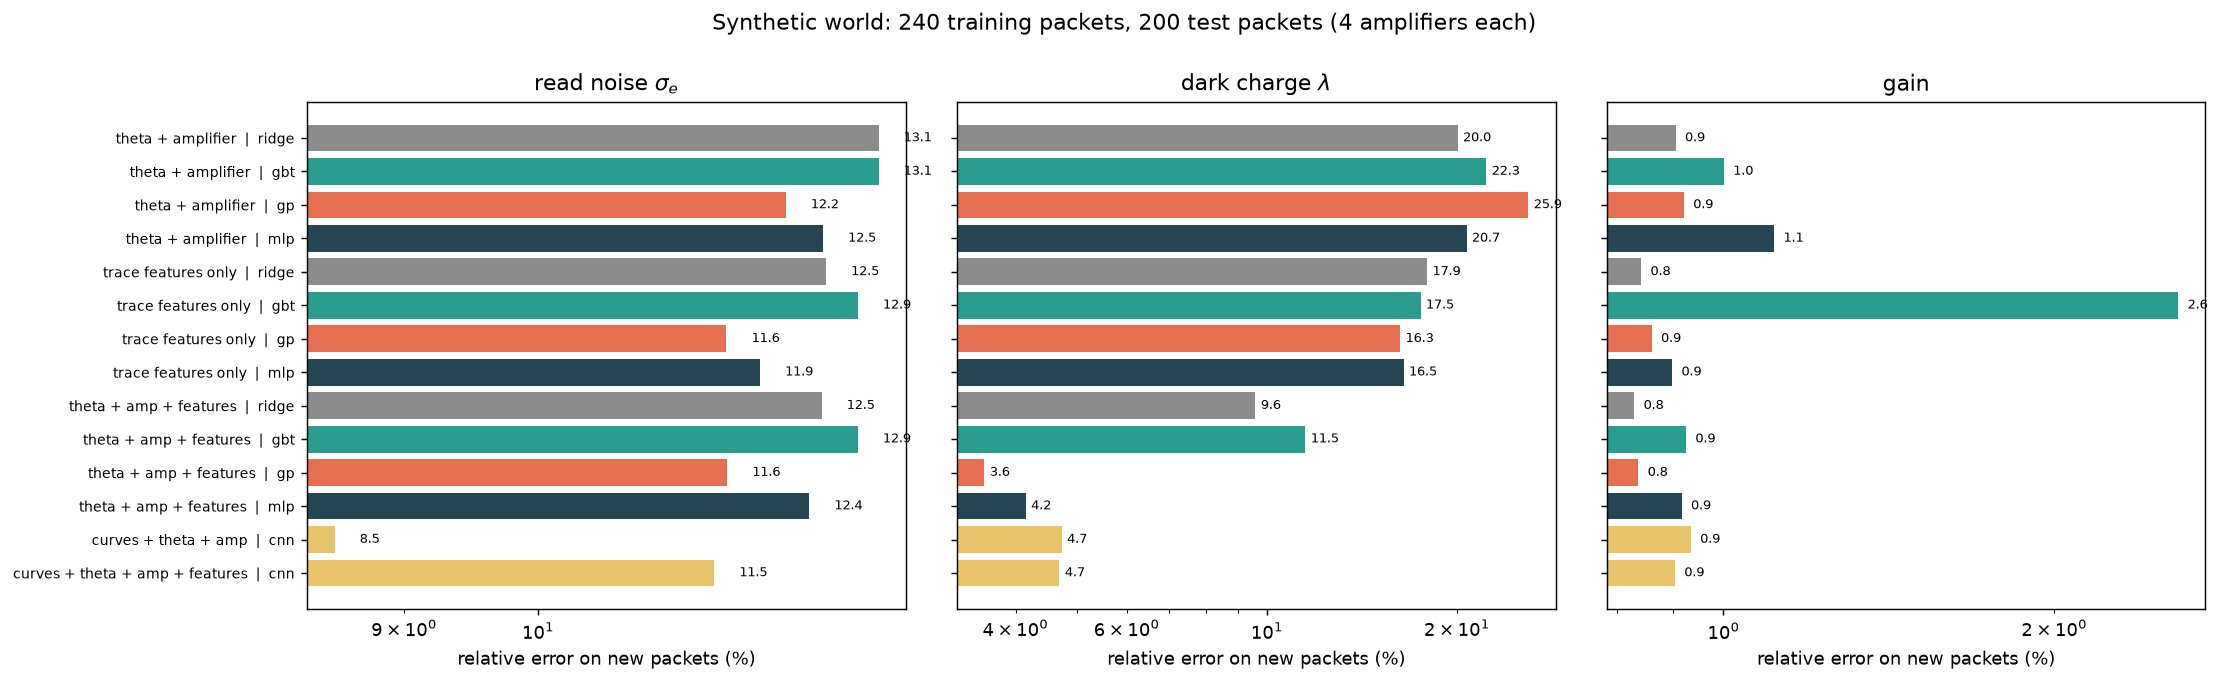
\includegraphics[width=\textwidth]{ml_inputs_models.png}
\caption{Relative error on 200 new packets, for each input set and model, after training on 240 packets (log scale).}
\label{fig:inputs}
\end{figure}

\begin{table}[H]
\centering
\small
\begin{tabular}{llccc}
\toprule
Inputs & Model & $\sigma_e$ & $\lambda$ & gain \\
\midrule
$\theta$ + amplifier & GP & 12.2\,\% & 25.9\,\% & 0.9\,\% \\
trace features only & GP & 11.6\,\% & 16.3\,\% & 0.9\,\% \\
$\theta$ + amplifier + features & GP & 11.6\,\% & \textbf{3.6\,\%} & 0.8\,\% \\
$\theta$ + amplifier + features & NN ensemble & 12.4\,\% & 4.2\,\% & 0.9\,\% \\
$\theta$ + amplifier + features & boosted trees & 12.9\,\% & 11.5\,\% & 0.9\,\% \\
curves + $\theta$ + amplifier & CNN & \textbf{8.5\,\%} & 4.7\,\% & 0.9\,\% \\
\bottomrule
\end{tabular}
\caption{Selected results of Figure~\ref{fig:inputs} (single training runs; differences of a few percent are within run-to-run variation).}
\end{table}

\begin{itemize}
\item \textbf{$\theta$ alone cannot predict $\lambda$} (26\,\%): the hidden drifting state changes $\lambda$ by $\pm35$\,\% and is not in $\theta$.
  The reference traces measure it: with the features, the GP reaches 3.6\,\%. This is the main reason to take reference traces in every packet.
\item \textbf{The gain} is set mostly by the amplifier and is easy for every model ($<1$\,\%, at the label noise).
\item \textbf{$\sigma_e$ is limited to about 12\,\% for every feature-based model}: the intermittent pickup adds a noise floor in 40\,\% of the
  packets, and no hand-made feature in the synthetic world describes it.
\item \textbf{Coverage}: the GP and the ensembles give calibrated error bars (coverage 0.67--0.80 for a target of 0.68). The boosted trees'
  quantile error bars are too narrow (0.4--0.6) with this little data; they are not suited to drive the optimizer.
\end{itemize}

\begin{figure}[H]
\centering
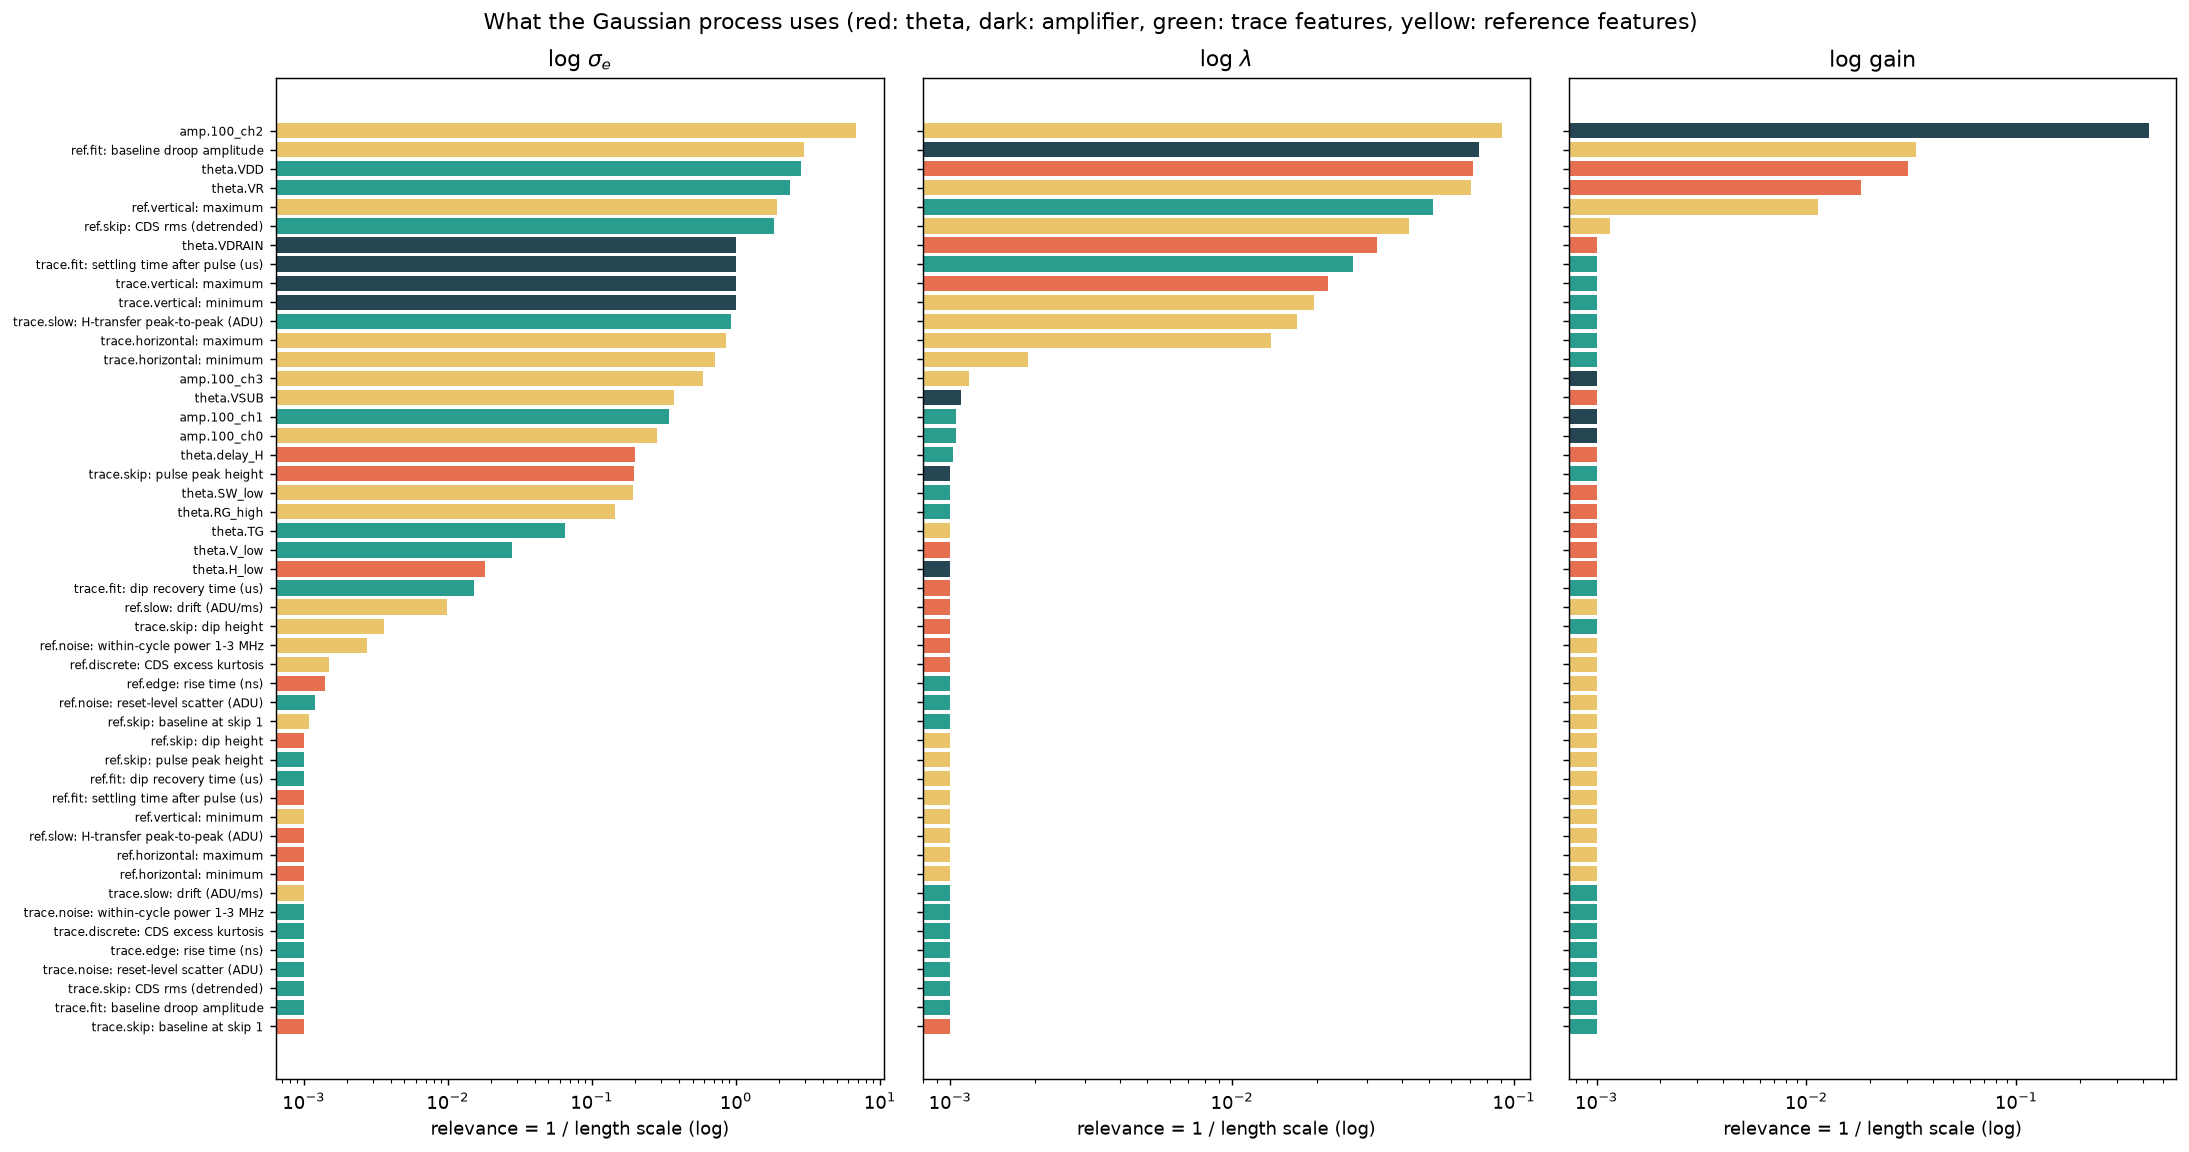
\includegraphics[width=\textwidth]{ml_gp_relevance.png}
\caption{Gaussian-process relevance ($1/\ell_i$) of every input, per target. The GP picks the physically right inputs: the CDS noise for $\sigma_e$,
the reference baseline (the hidden state) and the V low rails for $\lambda$, the amplifier for the gain.}
\label{fig:relevance}
\end{figure}

\subsection{How many packets}

\begin{figure}[H]
\centering
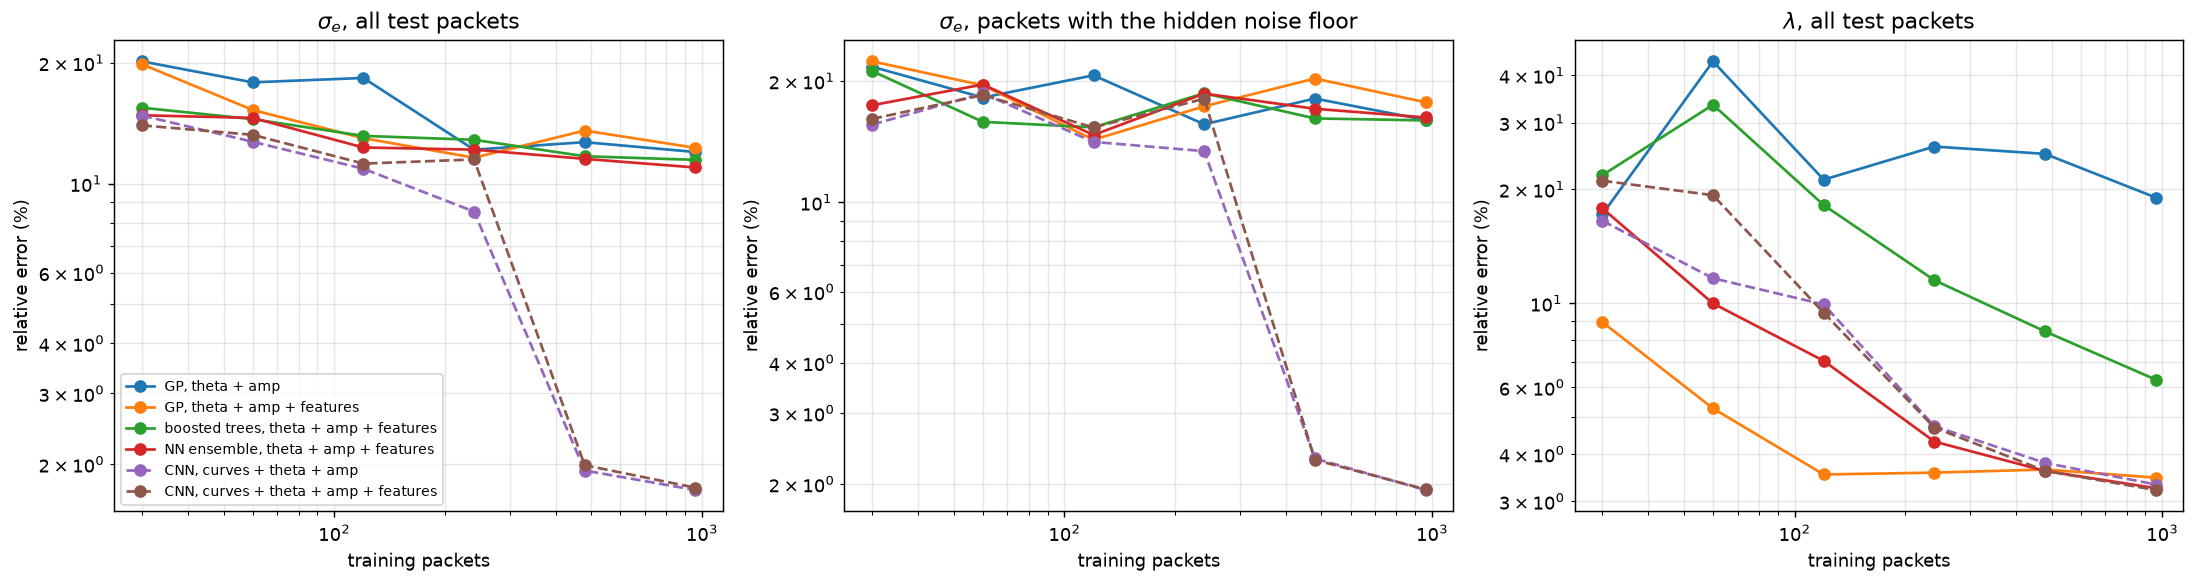
\includegraphics[width=\textwidth]{ml_learning_curves.png}
\caption{Error on new packets against the number of training packets. Middle: only the packets in which the hidden pickup was on.}
\label{fig:learning}
\end{figure}

\begin{itemize}
\item The \textbf{feature-based models level off} at about 11--12\,\% for $\sigma_e$ from $\sim$120 packets: more data does not help them see the
  pickup.
\item The \textbf{CNN on the curves} matches them up to $\sim$240 packets and then drops to \textbf{1.9\,\% at 480 and 1.7\,\% at 960 packets},
  also on the packets with pickup. It has \emph{found} the noise floor in the Allan-deviation and spectrum curves, without being told
  what to look for.
\item For $\lambda$, the GP with features is good from $\sim$60 packets (5\,\%) and reaches 3.5\,\%; the CNN reaches 3.3\,\% at 960.
\item \textbf{Lesson}: hand-made features win while data are scarce; a network on the curves overtakes them once there are several
  hundred labeled packets, if the curves hold something the features do not.
\end{itemize}

\subsection{Features, curves, or both?}
\label{sec:representation}

This is the question of Section~\ref{sec:fulltrace}, tested directly. Every candidate sees the traces at $\theta$ \emph{and} the reference
traces (as 30 numbers, as 14 curves, or both), so only the representation differs. Each is tested with and without $\theta$ + amplifier.

\begin{figure}[H]
\centering
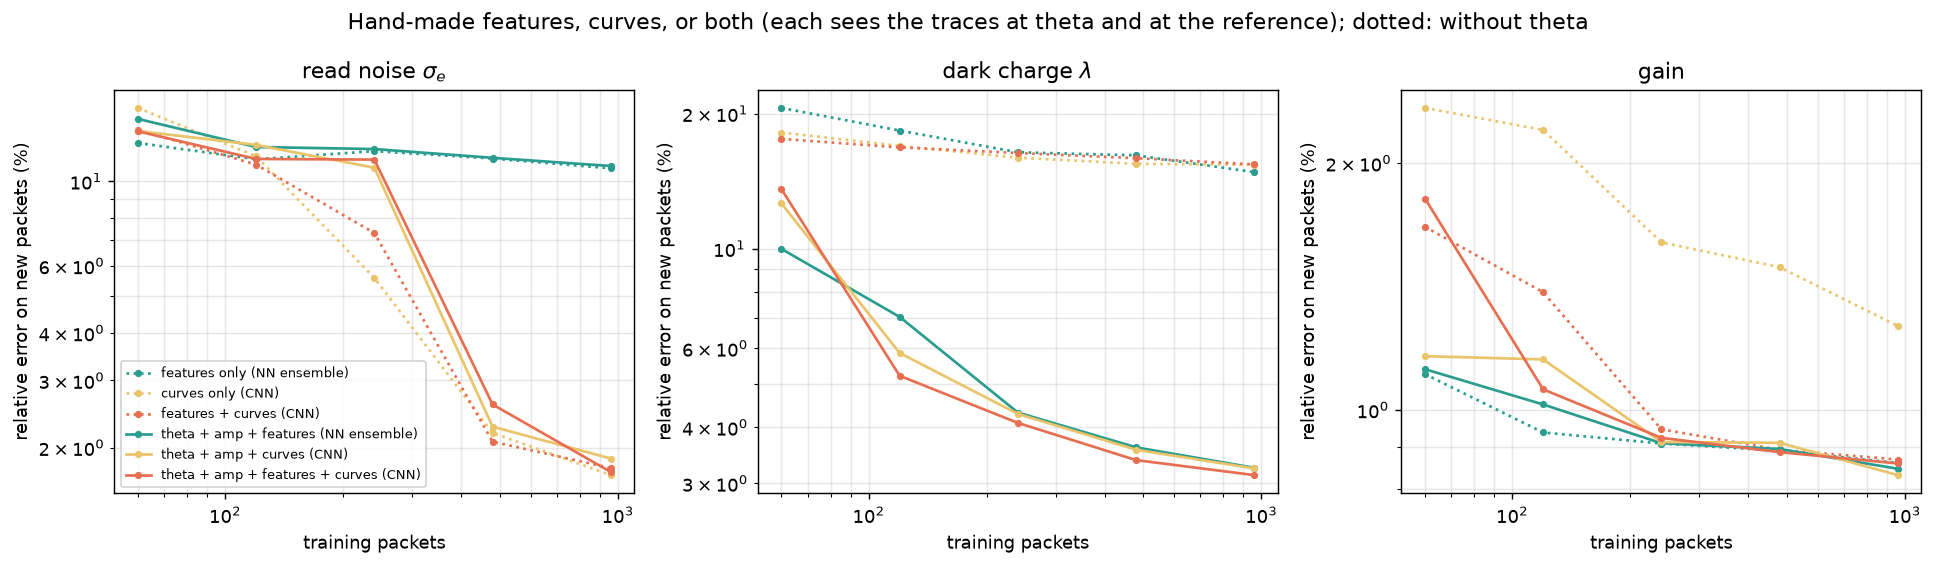
\includegraphics[width=\textwidth]{ml_representation.png}
\caption{Error on new packets against the number of training packets for the three representations; dotted: without $\theta$ + amplifier.}
\label{fig:representation}
\end{figure}

\begin{table}[H]
\centering
\small
\begin{tabular}{lcccccc}
\toprule
 & \multicolumn{3}{c}{$\sigma_e$} & \multicolumn{3}{c}{$\lambda$} \\
Inputs (all with the reference) & 120 & 480 & 960 & 120 & 480 & 960 \\
\midrule
$\theta$ + amp + features (NN ensemble) & 12.3 & 11.5 & 11.0 & 7.0 & 3.6 & 3.2 \\
$\theta$ + amp + curves (CNN) & 12.5 & 2.3 & 1.9 & 5.9 & 3.6 & 3.2 \\
$\theta$ + amp + features + curves (CNN) & 11.4 & 2.6 & 1.7 & 5.2 & 3.4 & 3.1 \\
features only, no $\theta$ & 11.4 & 11.5 & 10.8 & 18.3 & 16.1 & 14.8 \\
curves only, no $\theta$ & 11.6 & 2.2 & 1.7 & 16.9 & 15.5 & 15.4 \\
\bottomrule
\end{tabular}
\caption{Relative errors (\%) at 120, 480 and 960 training packets.}
\end{table}

\begin{itemize}
\item \textbf{$\theta$ must be an input.} Without it, $\lambda$ stays at $\sim$15\,\% for every representation: the dark charge depends on rails
  (substrate, V and H low levels) whose effect on $\lambda$ does not show in the traces.
\item \textbf{With little data} ($\le$120--240 packets) all representations are similar. The features are slightly better for $\lambda$ at
  60 packets, and the combination is the best or equal-best for $\lambda$ at every size.
\item \textbf{With enough data} (480+), the curves win for $\sigma_e$ (1.7--2.6\,\% against $\sim$11\,\%), because only they show the pickup
  floor. Adding the hand-made features to the curves neither helped nor hurt $\sigma_e$ much (within the run-to-run scatter), and helped
  $\lambda$ slightly.
\item \textbf{Answer:} give the model \textbf{$\theta$ + reference + both representations}. The features carry what we know matters and the
  absolute levels (which the curves remove), and make the model work with little data. The curves let it find what we did not think of
  once there are a few hundred packets. The trace alone (without $\theta$) is not enough, and the hand-made features alone cap the accuracy.
\end{itemize}


\subsection{A module never seen in training}

A second synthetic module (its own gain, noise and VDD optimum) was predicted by models trained on the first module plus 0, 5 or 20 of the
new module's packets:

\begin{table}[H]
\centering
\small
\begin{tabular}{lcccccc}
\toprule
 & \multicolumn{2}{c}{0 packets} & \multicolumn{2}{c}{5 packets} & \multicolumn{2}{c}{20 packets} \\
Model, inputs & $\sigma_e$ & gain & $\sigma_e$ & gain & $\sigma_e$ & gain \\
\midrule
GP, $\theta$ + amp & 62\,\% & 33\,\% & 16\,\% & 2.5\,\% & 15\,\% & 1.2\,\% \\
GP, $\theta$ + amp + features & 72\,\% & 35\,\% & 16\,\% & 2.5\,\% & 15\,\% & 1.2\,\% \\
trees, $\theta$ + amp & 67\,\% & 44\,\% & 63\,\% & 36\,\% & 5\,\% & 1.8\,\% \\
\bottomrule
\end{tabular}
\end{table}

With one module in training, \emph{no} model generalizes to a new one: the new module's gain and noise level lie outside everything seen.
A few packets of the new module are enough for the gain (5), and about 20 for $\sigma_e$. In practice: \textbf{start every new module or
amplifier with $\sim$20 packets around its reference}, and train on several modules before expecting transfer.

\subsection{Bayesian optimization}

\begin{figure}[H]
\centering
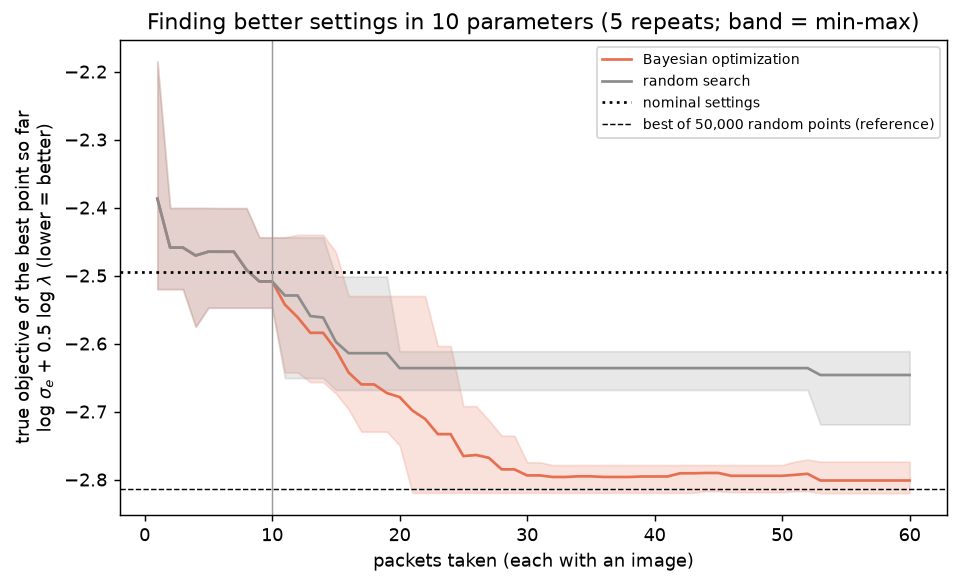
\includegraphics[width=0.8\textwidth]{ml_bo.png}
\caption{Best true objective found against the number of packets, for Bayesian optimization (after 10 random packets) and random search,
5 repeats each. Dotted: the nominal settings; dashed: the best of 50{,}000 random allowed settings.}
\label{fig:bo}
\end{figure}

With the GP surrogate and expected improvement, the optimizer came within 0.04 of the reference optimum ($J = -2.81$, against $-2.49$ at the
nominal settings; since $J=\log\sigma_e+\tfrac12\log\lambda$, $\sigma_e\sqrt\lambda$ is about 27\,\% lower) by 30 packets in all 5 repeats,
and ended at $-2.77$ to $-2.82$ after 60. Random search stalled at
$-2.61$ to $-2.72$ after 60 packets. In 10 dimensions a model-guided search needs a fraction of the packets of a random or grid scan.
On the real CCD the same loop runs with the limits and relations encoded, small steps, and a human approving each proposal at first.



%======================================================================
\section{What the first round taught us, and models to try next}
\label{sec:next}

The first models were chosen from the plan, before any were run. Running them exposed six specific weaknesses. Each points to a more
capable model.

\begin{table}[H]
\centering
\small
\begin{tabularx}{\textwidth}{>{\raggedright\arraybackslash}p{4.3cm}>{\raggedright\arraybackslash}p{4.4cm}X}
\toprule
Observed & Why & Model that addresses it \\
\midrule
1. Feature models plateau ($\sigma_e$ $\sim$12\,\%) & the hand-made features miss an effect & learned features (CNN); with little data: a \emph{deep-kernel GP} and \emph{pre-training} (C, D) \\
2. The CNN needs 300--500 labeled packets & it learns its features from the labels alone & self-supervised pre-training on the $\sim$30{,}000 unlabeled traces per scan (D) \\
3. A new module fails & nothing is shared across amplifiers and modules & hierarchical / multi-task GP; meta-learning (B, G) \\
4. Many inputs hurt the GP; tree error bars too narrow & one length scale per input over-fits; quantile trees are noisy & physics-structured outputs (A), deep kernels (C), conformal calibration (H) \\
5. Combining features and curves naively did not help the CNN & the network must learn to weigh 30 numbers against 7 curves & a fusion architecture with separate branches and per-feature noise (E) \\
6. One label per amplifier per packet & labels are expensive & more label information per image (per-row $\lambda$; A) and multi-fidelity use of trace-only packets (F) \\
\bottomrule
\end{tabularx}
\end{table}

\subsection*{A. Physics-structured outputs}
\begin{basic}
Instead of asking the model for $\sigma_e$ directly, ask for the pieces that physics combines: the single-skip noise, the noise floor, the
dark current and the clock-induced charge. The known formulas then give the labels. The model learns simpler things, and the result also
holds for a different number of skips or exposure time, which a black-box model cannot know.
\end{basic}
\begin{advanced}
Latent outputs $z(\theta, x) = (\log\sigma_1, \log\sigma_f, \log\text{DC}, \log\text{CIC}, \log g)$, with the observation model
\begin{equation}
\sigma_e^2 = \frac{\sigma_1^2}{N_\text{skip}} + \sigma_f^2,\qquad \lambda(r) = \text{CIC} + \text{DC}\,\bigl(E + r\,t_\text{row}\bigr),
\end{equation}
fitted by maximum likelihood to all available labels. The per-row $\lambda(r)$ of the 16-row image gives 16 constraints per amplifier
instead of 1, and the traces' block noise $\sigma(n)$ constrains $\sigma_1$ and $\sigma_f$ directly. Any regressor (GP, network) can sit
underneath.
\end{advanced}

\subsection*{B. Hierarchical and multi-task Gaussian processes}
\begin{basic}
Amplifiers and modules are different but related. A hierarchical model learns what they share and how much each one differs, so a new
module needs a few packets to learn its own offsets rather than a whole scan. It can also learn that $\sigma_e$, $\lambda$ and the gain
move together.
\end{basic}
\begin{advanced}
An intrinsic coregionalization kernel $k((\theta,a,t),(\theta',a',t')) = k_\theta(\theta,\theta')\,B^{\text{amp}}_{aa'}\,B^{\text{task}}_{tt'}$, or
additive amplifier random effects $f_a(\theta) = f(\theta) + \delta_a(\theta)$ with
$\delta_a \sim \mathcal{GP}(0, \sigma_\delta^2 k_\delta)$. A new module's offsets are then inferred from its first packets with calibrated
uncertainty. This is the principled fix for the held-out-module failure.
\end{advanced}

\subsection*{C. Deep kernel learning (a CNN inside a Gaussian process)}
\begin{basic}
The CNN finds new features but needs much data and gives less reliable error bars; the GP has honest error bars and needs little data
but only uses the inputs it is given. A deep kernel puts the CNN in front of the GP: the CNN turns the curves into a few learned numbers,
and the GP works on those. This combines both strengths, and it can serve as the optimizer's surrogate once traces are taken.
\end{basic}
\begin{advanced}
$k(x, x') = k_\text{Mat\'ern}\bigl(g_\phi(x), g_\phi(x')\bigr)$, with $g_\phi$ the convolutional encoder. The parameters $\phi$ and the GP
hyperparameters maximize the exact GP marginal likelihood jointly. With $n \lesssim 10^3$ exact inference is cheap. Over-fitting of
$\phi$ is controlled by pre-training (D), a small embedding (4--8 dimensions) and weight decay.
\end{advanced}

\subsection*{D. Self-supervised pre-training on unlabeled traces}
\begin{basic}
Every packet gives one image but 120 traces. A network can first learn ``what traces look like'' from all of them without labels, for
example by filling in hidden parts of the curves, or by recognizing that two repeats of the same packet belong together. It then needs
only a few labeled packets to learn what matters for the image.
\end{basic}
\begin{advanced}
Objectives:
\begin{itemize}
\item masked reconstruction of curves or folded cycles;
\item contrastive learning (InfoNCE) with positives = repeats of one packet and negatives = other packets;
\item prediction of $\theta$, which is known for every trace;
\item prediction of the reference from $\theta$ (state-invariant features).
\end{itemize}
The encoder then feeds (C) or a small supervised head. This is also the route to using the CDS matrix and the folded raw trace
(transformers over cycles, temporal convolution over skips).
\end{advanced}

\subsection*{E. Fusion and set models}
\begin{basic}
Today the repeats are averaged into one number per feature before the model sees them. A set model looks at all 10 repeats (and all
pixels) at once. It learns how much to trust each, ignores outliers by itself, and sees how much a feature scatters.
\end{basic}
\begin{advanced}
Separate branches for $\theta$, features (with their \code{trace\_sd} as inputs or as heteroscedastic noise) and curves, joined by a
gated or attention fusion layer. Permutation-invariant pooling (DeepSets, $\rho(\sum_i \psi(x_i))$, or attention pooling) over repeats
and pixels.
\end{advanced}

\subsection*{F. Multi-fidelity and better optimization}
\begin{advanced}
\begin{itemize}
\item \textbf{Multi-fidelity GP} (autoregressive co-kriging, $f_\text{image}(\theta) = \rho\,f_\text{trace}(\theta) + \delta(\theta)$) with a
  cost-aware acquisition. It decides between a $\sim$1-minute trace-only packet and a full 16-minute packet.
\item \textbf{Trust-region BO} (TuRBO) for 10--40 parameters.
\item \textbf{Constrained BO} with a learned feasibility model, where the limits are not known in closed form.
\item \textbf{Multi-objective acquisition} (expected hypervolume improvement) for the $\sigma_e$--$\lambda$ front.
\end{itemize}
The BoTorch/GPyTorch libraries implement these.
\end{advanced}

\subsection*{G, H. Few-shot transfer and calibrated error bars}
\begin{advanced}
\textbf{G}: neural processes or meta-learned GP priors, trained across modules, adapt to a new module from a handful of packets.
\textbf{H}: split-conformal calibration rescales any model's intervals on held-out packets so that their coverage is guaranteed
(distribution-free). It is cheap and fixes the trees' narrow intervals.
\end{advanced}

\subsection*{Priorities}
\begin{enumerate}
\item \textbf{A + B} (physics-structured outputs on a hierarchical GP). This needs the least data, transfers to new modules, and its
  predictions extrapolate in $N_\text{skip}$ and exposure. It is the best candidate for the first real scan.
\item \textbf{H} (conformal calibration) for every model: a few lines, and immediately useful.
\item \textbf{D + C} (pre-trained encoder with a GP head) once the first scan's 29{,}000 traces exist. This is the way to get the CNN's
  feature discovery at the GP's data needs.
\item \textbf{F} (multi-fidelity BO) once the predictor $P$ is shown to work on real data.
\end{enumerate}
Each will be tested the same way: synthetic world first, then the real scan, against the first-round models.

%======================================================================
\section{Prototypes of the next models (A, B, F, H)}
\label{sec:proto}

\begin{basic}
The four cheapest candidates of Section~\ref{sec:next} were built and tested on the synthetic world:
\begin{itemize}
\item \textbf{A}, a model that measures on the trace what it can (the single-skip noise and the noise floor) and learns only the rest;
\item \textbf{B}, a Gaussian process that knows the data come from amplifiers on modules;
\item \textbf{H}, a calibration of every model's error bars;
\item \textbf{F}, an optimizer that models the read noise and the dark charge separately.
\end{itemize}
Code: \code{src/ml/structured.py}, \code{calibrate.py}, \code{benchmark\_structured.py}; walkthrough:
\code{notebooks/ml\_structured\_models.ipynb}.

\textbf{Main results:} PROTO-SUMMARY-PLACEHOLDER
\end{basic}

\subsection{Two synthetic worlds}
World \textbf{v2} is the world of Section~\ref{sec:results}: the trace physics is complete. World \textbf{v3} adds two things.
\begin{itemize}
\item \textbf{A noise term only the image sees}, $\sigma_\text{lf} = 0.10\,(1 + 0.5\,(V_R+3)^2)(1 + 0.3\,\Delta t_H)$\,e$^-$: low-frequency
  noise over the 4.8-min image that a 0.2-s trace of 10 pixels cannot measure; on average 29\,\% of $\sigma_e$. A model built on the
  trace physics must learn it from the labels.
\item \textbf{$\lambda$ row by row.} With EXPOSURE 0 a pixel of row $r$ collects dark current while the rows below it are read:
  $\lambda_r = \text{CIC} + \text{DC}\,(r+\tfrac12)/8$, each row measured to 12\,\% (about 80 events in 1000 pixels). A line through the
  16 rows gives DC to 12\,\% and CIC to 26\,\%; their mean is the usual label (3\,\%).
\end{itemize}

\subsection{A: physics-structured outputs}
\begin{basic}
The trace measures the noise in ADU, both how it averages down with skips and the floor that does not. Only the gain, which converts ADU to
electrons, cannot be seen on a trace. So A takes the noise from the trace, learns the gain, and learns a small correction for what
the image sees and the trace does not. The dark charge is learned directly, or as dark current plus CIC when the image gives it
row by row.
\end{basic}
\begin{advanced}
A weighted least-squares fit of $\sigma_A(n)^2 = a^2/n + b^2$ to the trace's Allan deviation gives $a = \sigma_1 g$ and
$b = \sigma_\text{floor}\,g$ (on real data also the features ``skip: CDS rms'' and ``fit: correlated noise floor''). Then
\begin{equation}
\log\sigma_e = \tfrac12\log\Bigl(\frac{a^2}{N} + b^2\Bigr) - \log\hat g(x) + \hat r(x),\qquad
\lambda = e^{\hat f_\text{DC}(x)} + e^{\hat f_\text{CIC}(x)} \ \text{(or a GP on }\log\lambda),
\end{equation}
where $\hat g$, $\hat r$, $\hat f$ are GPs (ordinary for ``A'', hierarchical for ``A+B'') on $x = (\theta$, packet state vector$)$. The
residual is trained on $\log\sigma_e - \tfrac12\log(a^2/N+b^2) + \log g$ with the \emph{labeled} gain, so it is not polluted by gain
errors; the predicted variances add. The \textbf{packet state vector} is the reference features minus each amplifier's training average,
averaged over the packet's amplifiers: it measures the drift without the amplifier signatures and exists for an amplifier never seen.
With the true gain, the trace alone gives $\sigma_e$ to about 1\,\% in v2.
\end{advanced}

\subsection{B: hierarchical Gaussian process}
\begin{advanced}
An exact GP (PyTorch, float64, L-BFGS on the marginal likelihood) with
\begin{equation}
k(x,x') = s^2 M(x,x') + \mathbb{1}[m=m']\bigl(c_m^2 + s_m^2 M(x,x')\bigr) + \mathbb{1}[a=a']\bigl(c_a^2 + s_a^2 M(x,x')\bigr) + \sigma_n^2\,\mathbb{1}[x=x'],
\end{equation}
$M$ Matérn-5/2 with ARD length scales, $m$ the module and $a$ the amplifier. A new amplifier gets the shared function with the
offset variances in its error bar; its first packets move it, shrunk toward the shared function. With a single training module $c_m$ is
not identifiable and stays at its prior, so the error bars for a new module are conservative.
\end{advanced}

\subsection{Results}

\paragraph{Number of packets (Figure~\ref{fig:protolearn}).} PROTO-LEARNING-PLACEHOLDER

\begin{figure}[p]
\centering
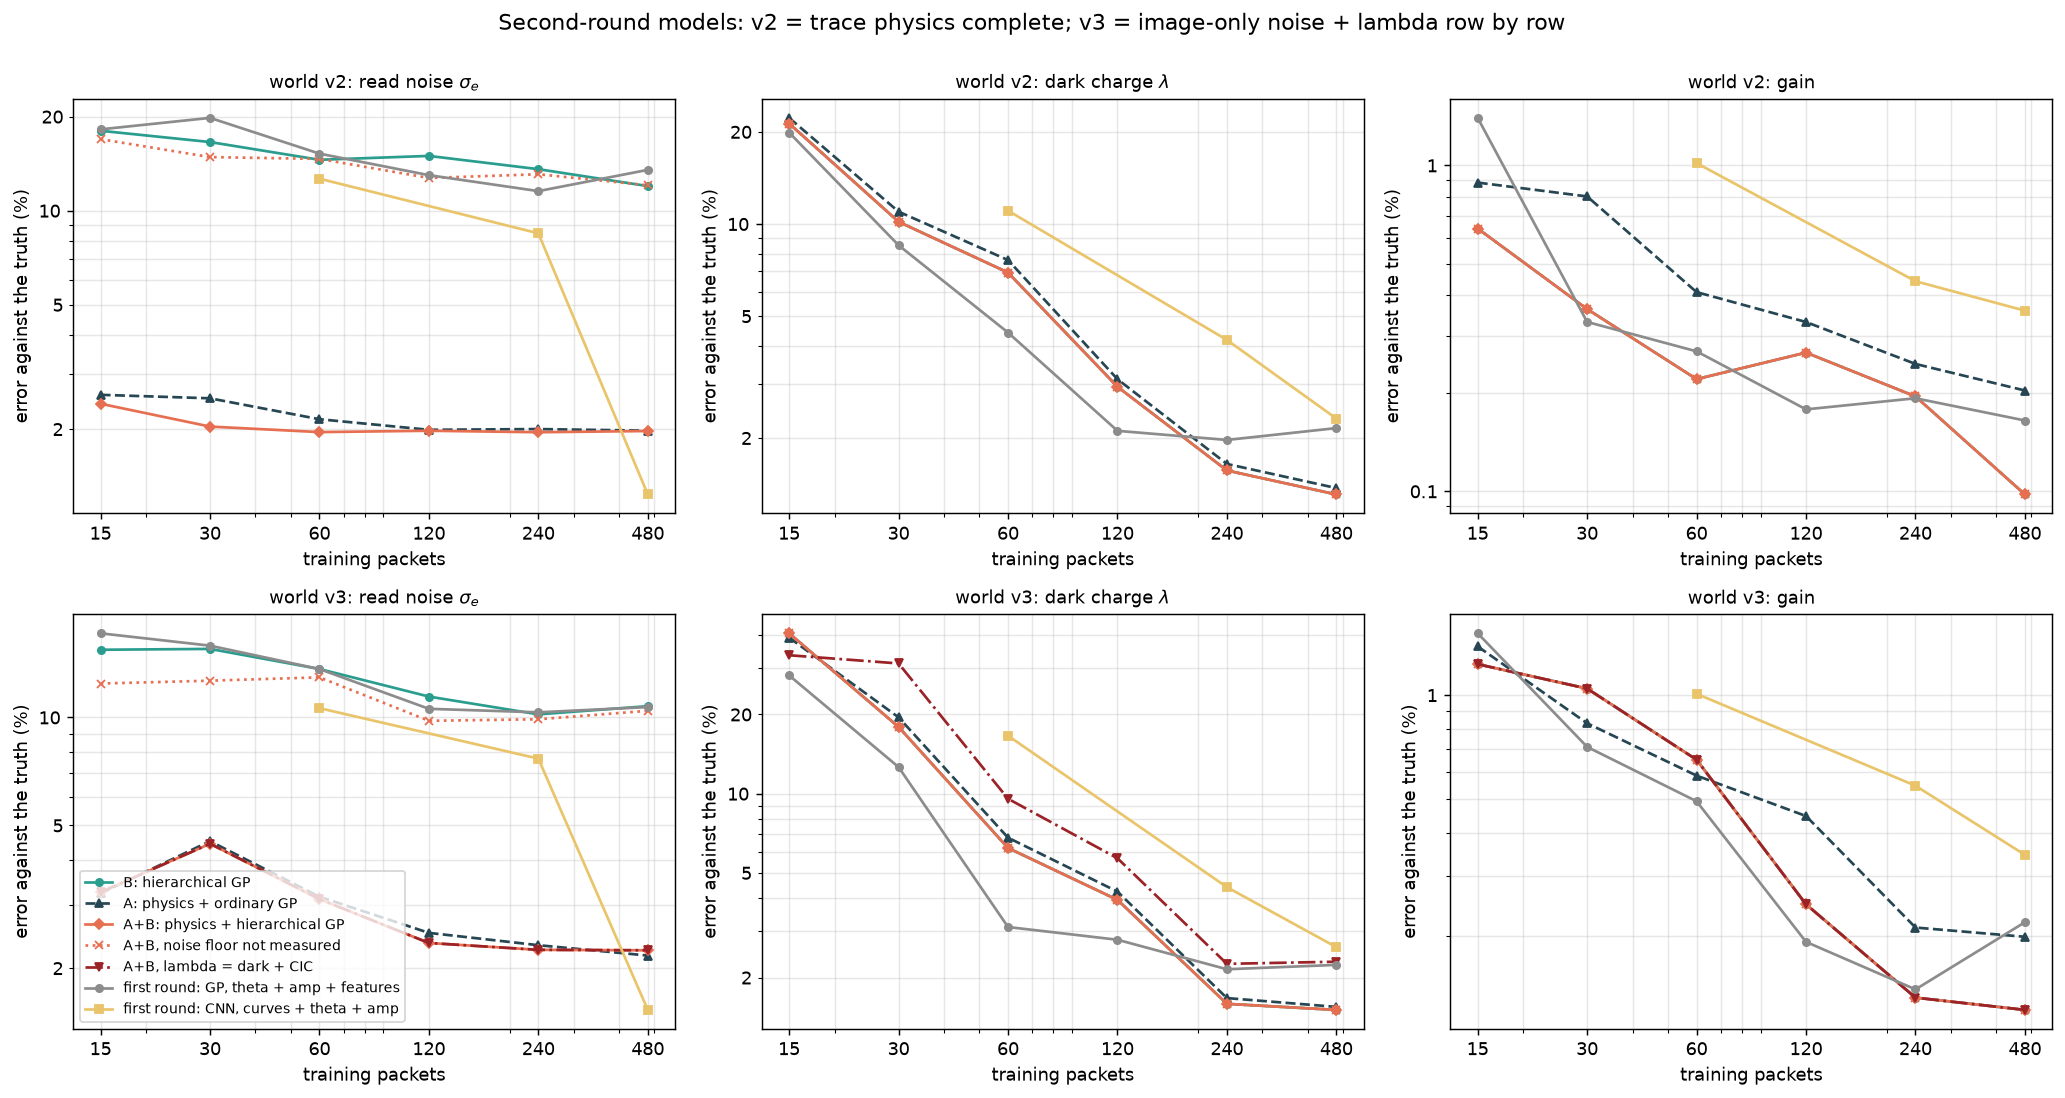
\includegraphics[width=\textwidth]{figures/ml_structured_learning.png}
\caption{Error against the noise-free truth on 200 new packets, against the number of training packets, in world v2 (top) and v3
(bottom). Grey: the first round's best feature model; yellow: the CNN on curves; red: A+B.}
\label{fig:protolearn}
\end{figure}

\paragraph{A new module (Figure~\ref{fig:protonew}).}
\begin{table}[h]
\centering\small
\begin{tabular}{lrrrrrr}
\toprule
& \multicolumn{3}{c}{$k=0$} & \multicolumn{3}{c}{$k=2$} \\
Model & $\sigma_e$ & $\lambda$ & gain & $\sigma_e$ & $\lambda$ & gain \\
\midrule
first round: GP, $\theta$ + amp + features & 72\,\% & 118\,\% & 35\,\% & 18\,\% & 39\,\% & 3.1\,\% \\
first round: boosted trees & 57\,\% & 50\,\% & 41\,\% & 38\,\% & 25\,\% & 20\,\% \\
B: hierarchical GP & 58\,\% & 3.6\,\% & 33\,\% & 7.4\,\% & 3.1\,\% & 0.9\,\% \\
A: physics + ordinary GP & 44\,\% & 3.1\,\% & 44\,\% & 2.6\,\% & 6.3\,\% & 1.5\,\% \\
A+B & 33\,\% & 3.6\,\% & 33\,\% & 2.4\,\% & 3.1\,\% & 0.9\,\% \\
\bottomrule
\end{tabular}
\caption{Error on a module never seen ($k=0$) or seen in 2 packets, after 240 packets of the first module (against the labels).}
\label{tab:protonew}
\end{table}
\begin{itemize}
\item With no packet of the new module, nothing can know its gain: the trace measures $\sigma_1 g$, never $g$. So $\sigma_e$ is off by the
  module-to-module gain spread for every model. Only the hierarchical GP says so: its coverage stays at 0.75, while A with an ordinary GP
  claims 0.00.
\item $\lambda$ does not depend on the module, and the state is read from the \emph{other} module's reference traces in the same packet:
  3\,\% instead of 50--118\,\%.
\item With \textbf{one} packet of the new module, A+B reaches $\sigma_e$ 3.3\,\%, $\lambda$ 3.1\,\%, gain 3.4\,\%; with two, 2.4/3.1/0.9\,\%.
  That is the level of a known module. The first round needed $\sim$20 packets. An ordinary GP is fragile here (A at $k=1$: $\lambda$
  37\,\%, an almost unseen one-hot column), the hierarchy is not.
\end{itemize}

\begin{figure}[p]
\centering
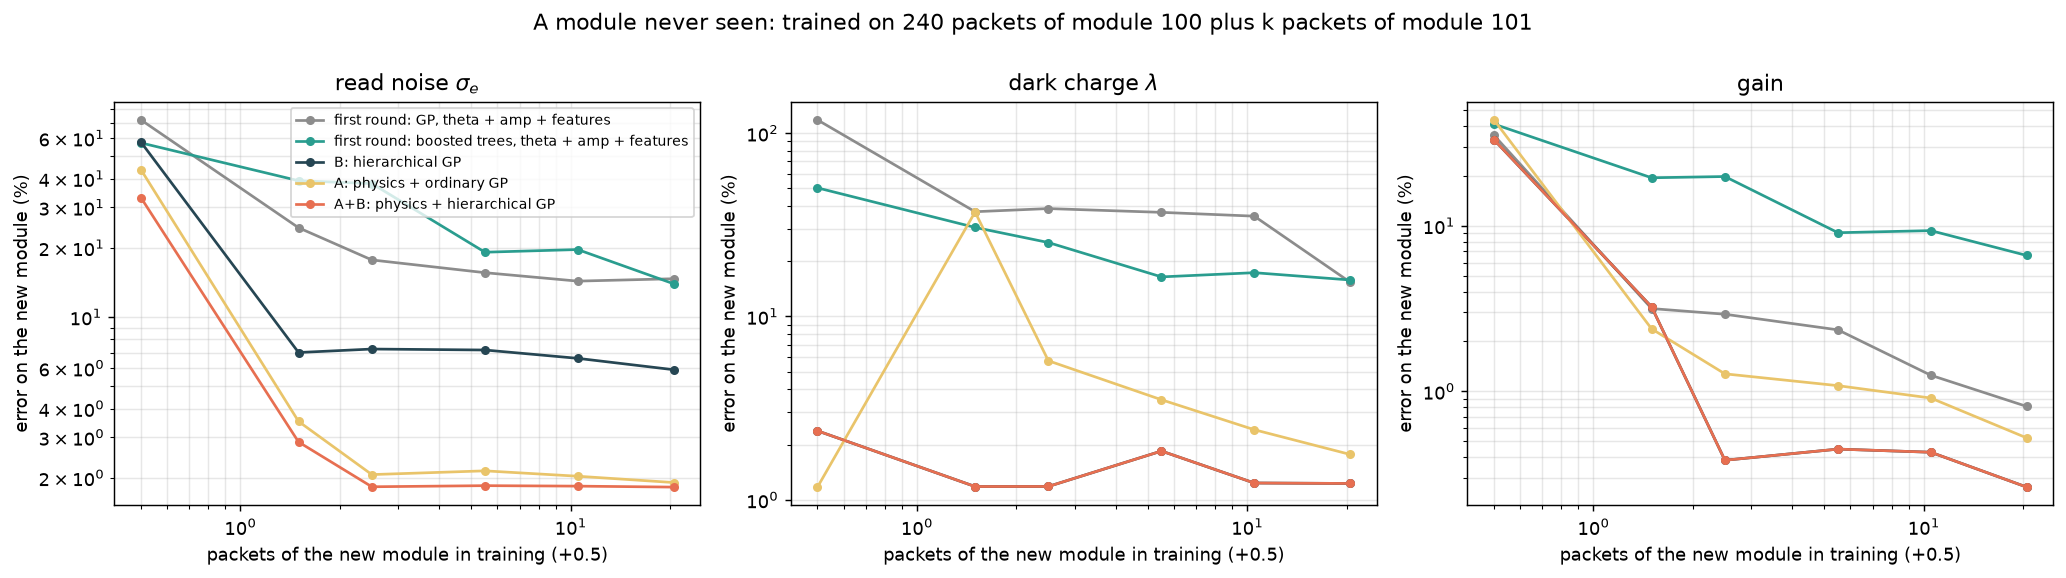
\includegraphics[width=\textwidth]{figures/ml_structured_newmodule.png}
\caption{Error on a new module against the number $k$ of its packets in training (plotted at $k+0.5$).}
\label{fig:protonew}
\end{figure}

\paragraph{Scan design.} PROTO-DESIGN-PLACEHOLDER

\paragraph{Calibrated error bars (H).} PROTO-CONFORMAL-PLACEHOLDER

\paragraph{Decomposed surrogate for optimization (F; Figure~\ref{fig:protobo}).} Two hierarchical GPs model $\log\sigma_e$ and $\log\lambda$
per good amplifier, and $J$ is computed from them (its variance assuming fully correlated amplifiers). Each part depends on fewer
parameters than $J$, so it is learned from fewer packets. Over 5 repeats, the best true $J$ after 30 packets is $-2.80$ to $-2.82$
(decomposed) against $-2.75$ to $-2.79$ (one GP on $J$). After 60 packets both reach $-2.80$ to $-2.82$ (the best of 50{,}000 random
points: $-2.81$). Decomposing does not find a better optimum; it finds it in about half the packets.

\begin{figure}[h]
\centering
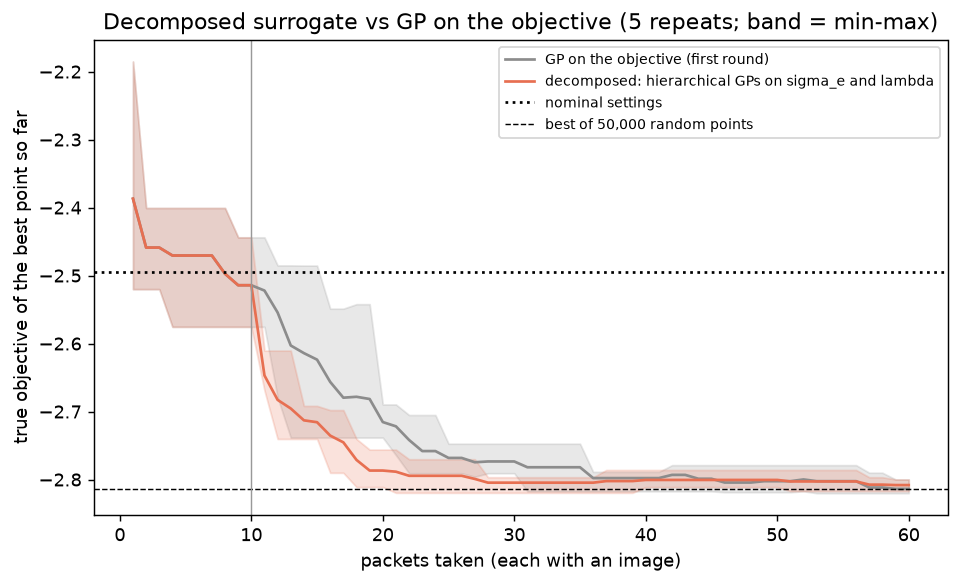
\includegraphics[width=0.7\textwidth]{figures/ml_structured_bo.png}
\caption{Best true objective against the number of packets: one GP on $J$ (grey) and the decomposed surrogate (red), 5 repeats.}
\label{fig:protobo}
\end{figure}

\paragraph{C, D, E on the synthetic world.} They are not tested here, on purpose. In this world A+B already uses everything the curves
contain (the floor in the Allan deviation), and the image-only term is invisible to the traces by construction, so a learned encoder
cannot show a gain. Whether the real curves contain effects that A's physics misses can only be tested on real data (stage 4 of
Section~\ref{sec:realtest}).

%======================================================================
\section{Testing every model on real data}
\label{sec:realtest}

\begin{basic}
The synthetic world only ranks methods. On the real CCD the models are tested in stages, each stage using data that the packets
produce anyway, and each with a test that a model cannot pass by memorizing. Stage 0 needs no training at all: it checks whether the
physics that model A relies on holds on our CCD.
\end{basic}

\paragraph{Stage 0 -- the first packets at nominal settings (no training).}
\begin{itemize}
\item \textbf{Label noise.} Repeat the nominal packet $\gtrsim$5 times: the scatter of WADERs' $\sigma_e$, $\lambda$ and gain between repeats is the
  floor no model can beat (synthetic: 1.5\,\%, 3\,\%, 0.8\,\%). Compare with WADERs' own error bars (\code{sigma\_e\_err}, \code{lambda\_err}).
\item \textbf{Does the trace physics hold?} With the gain from the image, the trace alone predicts
  $\sigma_e^\text{trace} = \sqrt{a^2/N + b^2}/g$ ($a, b$ from the Allan deviation, or the features ``skip: CDS rms'' and
  ``fit: correlated noise floor''). The ratio $\sigma_e^\text{image}/\sigma_e^\text{trace}$ and its scatter decide how much model A must
  learn: a ratio near 1 with small scatter means A works almost without training (world v2); a ratio that depends on the settings
  is what A's residual $r(x)$ learns (world v3).
\item \textbf{Dark current vs CIC.} Fit $\lambda$ row by row (16 rows): the slope is the dark current accumulated while the rows wait, the
  intercept the CIC. A clear slope means the per-row labels are worth adding to the dataset.
\end{itemize}

\paragraph{Stage 1 -- the first scan.} All models of both rounds, the same splits and scores:
\begin{itemize}
\item \textbf{splits:} (i) grouped by packet (5 folds); (ii) \emph{blocked in time}: train on the first 2/3 of the scan, test on the last
  1/3 (does the model follow the drift?); (iii) \emph{leave one parameter out} for a one-at-a-time scan: train on 9 parameters' sweeps
  and the references, test on the 10th (it measures what the model can \emph{not} know, and is the honest test for a design without joint
  changes);
\item \textbf{scores:} relative error against the labels, compared with the label noise of stage 0; coverage of the 68\,\% and 95\,\%
  intervals before and after conformal calibration (H); for the surrogate, the rank correlation between the predicted and measured
  objective and the regret of the best predicted point;
\item \textbf{learning curves:} the same, on random subsets of 15, 30, 60, 120, 240 packets;
\item \textbf{what the models use:} GP relevances, A's residual $r(x)$ (where the trace physics fails), and, for the CNN, which parts of the
  curves matter (saliency).
\end{itemize}

\paragraph{Stage 2 -- a second module (when one is available).} Train on module 1 plus $k = 0, 1, 2, 5, 10, 20$ packets of module 2;
test on its other packets (the \code{newmodule} experiment). This decides B against the first round and how many packets a new module needs.

\paragraph{Stage 3 -- the optimizer.} First \emph{offline}: replay Bayesian optimization on the scan, choosing only among the measured
packets (pool-based), for every surrogate; cheap and fair. Then one \emph{prospective} run with the best surrogate: it proposes, we take the
packet, and the prediction made before the packet is compared with the result. Only this last test measures what we care about.

\paragraph{Stage 4 -- the data-hungry models (C, D, E, F).} Once there are tens of thousands of traces: pre-train the encoder on all of them
(D), put it under the GP (C), and compare with A+B at the same number of labeled packets. Set models (E) need the individual trace sets
(see the data format below).

%======================================================================
\section{Do the packets need to change?}
\label{sec:dataneeds}

\begin{basic}
Mostly no: the packet as designed (5 reference sets, 10 trace sets, one 16-row image) carries what every model needs. Four additions
would make the models clearly better, and one choice in the scan design matters a lot. None of them makes a packet longer.
\end{basic}

\begin{table}[h]
\centering\small
\begin{tabularx}{\textwidth}{>{\raggedright\arraybackslash}p{4.3cm}>{\raggedright\arraybackslash}X>{\raggedright\arraybackslash}p{2.4cm}}
\toprule
Change & Why (which model) & Cost \\
\midrule
\textbf{Per-row $\lambda$ from WADERs} (and per-row $\sigma$) & splits dark current from CIC (A); 16 constraints per image instead of 1; was already an
  open item (WADERs JSON with per-row dark current) & none (analysis only) \\
\textbf{Keep the un-averaged skips of the image}, or of a few of its rows, if the DAQ can save them & the image's own $\sigma(N)$ curve: $\sigma_1$,
  floor and the image-only noise measured on the image, not inferred (A; stage 0) & disk (tens of MB per channel for 16 rows; check that cdaq can save them) \\
\textbf{A scan design with joint changes}: random/Sobol points inside the limits, or half one-at-a-time and half random & the
  one-at-a-time design never changes two parameters together, so no model can learn interactions (the \code{design} experiment, below) & none
  (same number of packets) \\
\textbf{Trace-only packets} between the image packets, at extra settings & unlabeled traces for pre-training (D), the cheap fidelity of
  multi-fidelity BO (F), and many more $\theta$ points for the trace physics $a(\theta), b(\theta)$ (A) & minutes each, no image \\
\textbf{Record the conditions}: CCD and board temperatures, time since the last flush/erase, vacuum, the complete parameter set of every pin
  (not only the scanned ones), software versions & the drifting state is today inferred from the reference traces; measured temperatures
  make it direct (all models; B for modules) & none \\
\textbf{Nominal image packets at intervals} (the scan already has \code{reference\_every = 5}) & labeled drift anchors: they measure the
  state's effect on the labels directly & already planned \\
\textbf{A few packets of every new module}, at nominal and around it & B needs $\gtrsim$2--5 imaged packets per new module before its gain
  (and so $\sigma_e$) is known; traces alone cannot give the gain & 2--5 packets \\
\bottomrule
\end{tabularx}
\caption{Changes to the data that the second-round models would use. None makes a packet longer.}
\label{tab:dataneeds}
\end{table}

%======================================================================
\section{A better data format}
\label{sec:format}

\begin{basic}
Today the models read \code{dataset.csv}: one row per packet and amplifier, every feature already averaged over the repeats. That is
the right table for the first-round models, but it throws away what the next ones need: the individual repeats, the curves, the label
error bars, the row-by-row image information and the conditions. The proposal is to keep the raw files as they are and add a small set
of linked tables, from which \code{dataset.csv} is just one view.
\end{basic}

\begin{advanced}
\textbf{Keep} the raw data as the source of truth (FITS images, lossless \code{.npz} traces, \code{result.json}). \textbf{Add} a tidy,
columnar store (Parquet tables plus one array store, HDF5 or Zarr), keyed by \code{packet\_id}, \code{board}, \code{channel}, \code{kind}
(reference / $\theta$) and \code{set}:
\begin{enumerate}
\item \code{packets}: time stamps, module and CCD identifiers, configuration hashes, the complete parameter vector (every pin),
  temperatures and other conditions, readout times, flags; also the trace-only packets;
\item \code{trace\_sets}: one row per trace set (not combined): quality flags and all 85 features, so that set models (E) and robust
  combinations can be learned, and the repeat scatter is a feature in its own right;
\item \code{curves}: the 12 curves of every trace set, at their natural length (array store), for the CNN, pre-training (D) and deep kernels (C);
\item \code{labels}: per packet and amplifier $\sigma_e$, $\lambda$, gain \emph{with their errors} (for heteroscedastic likelihoods: the GP
  then uses WADERs' error instead of learning one noise level), fit flags, WADERs version;
\item \code{image\_rows}: per row (and column) $\lambda$, $\sigma$, baseline: the information model A uses; and, if available, the image's own
  $\sigma(N)$ curve;
\item \code{schema}: version and the hash of the code that produced every table.
\end{enumerate}
\code{dataset.csv} becomes a derived view (combine the sets, join the labels), so the first-round code is unchanged. Trace-only packets
are rows without labels; new modules are new identifiers. Loading one table into pandas or PyTorch is a single call.
\end{advanced}

%======================================================================
\section{Plan}

\begin{enumerate}
\item \textbf{Now (no labels yet):} the pipeline runs end to end on synthetic data (\code{python -m ml.benchmark}). The real
  \code{dataset.csv} loads with \code{ml.data.load\_dataset}, and the curves with \code{curves\_from\_processed}.
\item \textbf{First real packets:} check the label noise and the repeat scatter; fit the GP surrogate on the first tens of packets;
  check the coverage on held-out packets.
\item \textbf{First scan (241 packets):}
  \begin{itemize}
  \item compare ridge, trees, GP and the neural-net ensemble on the hand-made features (grouped CV and a second night);
  \item read the GP relevances;
  \item test the held-out amplifier.
  \end{itemize}
\item \textbf{CNN on curves:} train it on the same scan; pre-train an encoder on all unlabeled traces; compare; look at what it uses.
\item \textbf{Next models:} A+B, H and F are prototyped (Section~\ref{sec:proto}); deep kernel with pre-training (C+D) and set models (E)
  wait for real traces. The real-data test plan is in Section~\ref{sec:realtest}.
\item \textbf{Optimization:} Bayesian optimization in the screened parameters, with the limits and relations encoded, small steps and
  human approval of each proposal at first.
\end{enumerate}

\paragraph{Software.}
\begin{itemize}
\item \code{src/ml/}: \code{synthetic.py}, \code{data.py}, \code{models.py}, \code{evaluate.py}, \code{optimize.py}, \code{benchmark.py},
  and the plots; second round: \code{structured.py}, \code{calibrate.py}, \code{benchmark\_structured.py}.
\item Notebooks: \code{notebooks/ml\_models\_walkthrough.ipynb} (first round), \code{notebooks/ml\_structured\_models.ipynb} (second round).
\item Environment: \code{python3 -m venv .venv \&\& .venv/bin/pip install -r requirements-ml.txt} (numpy, scipy, pandas, scikit-learn,
  PyTorch, matplotlib).
\item The benchmarks: \code{cd src \&\& ../.venv/bin/python -m ml.benchmark} and \code{-m ml.benchmark\_structured}.
\end{itemize}

\end{document}
